% Options for packages loaded elsewhere
\PassOptionsToPackage{unicode}{hyperref}
\PassOptionsToPackage{hyphens}{url}
\PassOptionsToPackage{dvipsnames,svgnames,x11names}{xcolor}
%
\documentclass[twoside]{extreport}
\usepackage{report-generic}
\usepackage{report-language}
% Alter some LaTeX defaults for better treatment of figures:
% See p.105 of "TeX Unbound" for suggested values.
% See pp. 199-200 of Lamport's "LaTeX" book for details.
%   General parameters, for ALL pages:
\renewcommand{\topfraction}{0.9}	% max fraction of floats at top
\renewcommand{\bottomfraction}{0.8}	% max fraction of floats at bottom
%   Parameters for TEXT pages (not float pages):
\setcounter{topnumber}{2}
\setcounter{bottomnumber}{2}
\setcounter{totalnumber}{4}     % 2 may work better
\setcounter{dbltopnumber}{2}    % for 2-column pages
\renewcommand{\dbltopfraction}{0.9}	% fit big float above 2-col. text
\renewcommand{\textfraction}{0.07}	% allow minimal text w. figs
%   Parameters for FLOAT pages (not text pages):
\renewcommand{\floatpagefraction}{0.7}	% require fuller float pages
% N.B.: floatpagefraction MUST be less than topfraction !!
\renewcommand{\dblfloatpagefraction}{0.7}	% require fuller float pages
\pagenumbering{arabic}

\usepackage[colorspec=0.9, fontsize=0.1\paperwidth, angle=90, hpos=5mm, anchor=lm]{draftwatermark}
\DraftwatermarkOptions{text={This is a watermark}}

\title{Analysis kartering}
\citationtitle{Analysis kartering}
\titleauthor{Robrecht Dockx, Hans Van Calster, Third Author}
\displaycolophon{1}
\colophonauthor{\href{https://orcid.org/0000-0002-1825-0097}{Robrecht Dockx
\includegraphics[height=\fontsizebase]{orcid.eps}}, \href{https://orcid.org/0000-0002-1825-0098}{Hans Van Calster
\includegraphics[height=\fontsizebase]{orcid.eps}}, \href{https://orcid.org/0000-0002-1825-0097}{Third Author
\includegraphics[height=\fontsizebase]{orcid.eps}}}
\colophonauthortag{Auteurs}
\reviewer{\href{https://orcid.org/0000-0002-1825-0097}{First Reviewer
\includegraphics[height=\fontsizebase]{orcid.eps}}}
\reviewertag{Reviewers}
\missiontag{Het INBO is het onafhankelijk onderzoeksinstituut van de
Vlaamse overheid dat via toegepast wetenschappelijk onderzoek, data- en
kennisontsluiting het biodiversiteitsbeleid en -beheer onderbouwt en
evalueert.}
\entityname{Instituut voor Natuur- en Bosonderzoek}
\entityaddress{INBO Brussel, Herman Teirlinckgebouw, Havenlaan 88 bus
73, 1000 Brussel}
\locationtag{Vestiging}
\tagline{vlaanderen-wetenschap.pdf}
\definecolours{inbo}
\entityurl{https://www.vlaanderen.be/inbo}
\entityurltext{vlaanderen.be/inbo}
\doi{10.5281/zenodo.842223}
\ordernumber{optional order number}
\pagefootmessage{10.5281/zenodo.842223}
\public{1}
\corresponding{\href{mailto:robrecht.dockx@inbo.be}{robrecht.dockx@inbo.be} }
\country{België}
\citationtag{Wijze van citeren}
\shortauthor{ Dockx, R. et al.}
\citationyear{9999}
\reportnr{3.14}
\depotnr{optional depot number}
\seriestag{Rapporten van het}
\iseriestag{Interne rapporten van het}
\city{Brussel}
\issn{1782-9054}
\vu{Verantwoordelijke uitgever}
\vuname{Hilde Eggermont}
\covertag{Foto cover}
\coverdescription{Detail of a leaf. Photo by
\href{https://www.pexels.com/nl-nl/@skyler-ewing-266953?utm_content=attributionCopyText&utm_medium=referral&utm_source=pexels}{Skyler
Ewing} via
\href{https://www.pexels.com/nl-nl/foto/hout-natuur-rood-creatief-4599227/?utm_content=attributionCopyText&utm_medium=referral&utm_source=pexels}{Pexels}}
\client{\textbf{Dit onderzoek werd uitgevoerd in opdracht van:}\\INBO Brussel\\VAC Brussel ‐ Herman Teirlinck\\Havenlaan 88 bus 73\\1000 Brussel\\
\url{https://www.vlaanderen.be/inbo/en-gb}}
\cooperation{\textbf{Dit onderzoek werd uitgevoerd in samenwerking met:}\\INBO Brussel\\VAC Brussel ‐ Herman Teirlinck\\Havenlaan 88 bus 73\\1000 Brussel\\
\url{https://www.vlaanderen.be/inbo/en-gb}}
\ccby{Dit werk valt onder een \href{https://creativecommons.org/licenses/by/4.0/}{Creative Commons Naamsvermelding 4.0 Internationaal-licentie}.}
\titlelogo{
\includegraphics[height = 17mm, keepaspectratio]{inbo-logo.pdf}}


\usepackage{amsmath,amssymb}
\usepackage{iftex}
\ifPDFTeX
  \usepackage[T1]{fontenc}
  \usepackage[utf8]{inputenc}
  \usepackage{textcomp} % provide euro and other symbols
\else % if luatex or xetex
  \usepackage{unicode-math}
  \defaultfontfeatures{Scale=MatchLowercase}
  \defaultfontfeatures[\rmfamily]{Ligatures=TeX,Scale=1}
\fi
\usepackage{lmodern}
\ifPDFTeX\else  
    % xetex/luatex font selection
    \setmainfont[]{Calibri}
    \setmonofont[]{Inconsolatazi4}
\fi
% Use upquote if available, for straight quotes in verbatim environments
\IfFileExists{upquote.sty}{\usepackage{upquote}}{}
\IfFileExists{microtype.sty}{% use microtype if available
  \usepackage[]{microtype}
  \UseMicrotypeSet[protrusion]{basicmath} % disable protrusion for tt fonts
}{}
\makeatletter
\@ifundefined{KOMAClassName}{% if non-KOMA class
  \IfFileExists{parskip.sty}{%
    \usepackage{parskip}
  }{% else
    \setlength{\parindent}{0pt}
    \setlength{\parskip}{6pt plus 2pt minus 1pt}}
}{% if KOMA class
  \KOMAoptions{parskip=half}}
\makeatother
\usepackage{xcolor}
\setlength{\emergencystretch}{3em} % prevent overfull lines
\setcounter{secnumdepth}{5}
% Make \paragraph and \subparagraph free-standing
\makeatletter
\ifx\paragraph\undefined\else
  \let\oldparagraph\paragraph
  \renewcommand{\paragraph}{
    \@ifstar
      \xxxParagraphStar
      \xxxParagraphNoStar
  }
  \newcommand{\xxxParagraphStar}[1]{\oldparagraph*{#1}\mbox{}}
  \newcommand{\xxxParagraphNoStar}[1]{\oldparagraph{#1}\mbox{}}
\fi
\ifx\subparagraph\undefined\else
  \let\oldsubparagraph\subparagraph
  \renewcommand{\subparagraph}{
    \@ifstar
      \xxxSubParagraphStar
      \xxxSubParagraphNoStar
  }
  \newcommand{\xxxSubParagraphStar}[1]{\oldsubparagraph*{#1}\mbox{}}
  \newcommand{\xxxSubParagraphNoStar}[1]{\oldsubparagraph{#1}\mbox{}}
\fi
\makeatother

\usepackage{color}
\usepackage{fancyvrb}
\newcommand{\VerbBar}{|}
\newcommand{\VERB}{\Verb[commandchars=\\\{\}]}
\DefineVerbatimEnvironment{Highlighting}{Verbatim}{commandchars=\\\{\}}
% Add ',fontsize=\small' for more characters per line
\usepackage{framed}
\definecolor{shadecolor}{RGB}{241,243,245}
\newenvironment{Shaded}{\begin{snugshade}}{\end{snugshade}}
\newcommand{\AlertTok}[1]{\textcolor[rgb]{0.68,0.00,0.00}{#1}}
\newcommand{\AnnotationTok}[1]{\textcolor[rgb]{0.37,0.37,0.37}{#1}}
\newcommand{\AttributeTok}[1]{\textcolor[rgb]{0.40,0.45,0.13}{#1}}
\newcommand{\BaseNTok}[1]{\textcolor[rgb]{0.68,0.00,0.00}{#1}}
\newcommand{\BuiltInTok}[1]{\textcolor[rgb]{0.00,0.23,0.31}{#1}}
\newcommand{\CharTok}[1]{\textcolor[rgb]{0.13,0.47,0.30}{#1}}
\newcommand{\CommentTok}[1]{\textcolor[rgb]{0.37,0.37,0.37}{#1}}
\newcommand{\CommentVarTok}[1]{\textcolor[rgb]{0.37,0.37,0.37}{\textit{#1}}}
\newcommand{\ConstantTok}[1]{\textcolor[rgb]{0.56,0.35,0.01}{#1}}
\newcommand{\ControlFlowTok}[1]{\textcolor[rgb]{0.00,0.23,0.31}{\textbf{#1}}}
\newcommand{\DataTypeTok}[1]{\textcolor[rgb]{0.68,0.00,0.00}{#1}}
\newcommand{\DecValTok}[1]{\textcolor[rgb]{0.68,0.00,0.00}{#1}}
\newcommand{\DocumentationTok}[1]{\textcolor[rgb]{0.37,0.37,0.37}{\textit{#1}}}
\newcommand{\ErrorTok}[1]{\textcolor[rgb]{0.68,0.00,0.00}{#1}}
\newcommand{\ExtensionTok}[1]{\textcolor[rgb]{0.00,0.23,0.31}{#1}}
\newcommand{\FloatTok}[1]{\textcolor[rgb]{0.68,0.00,0.00}{#1}}
\newcommand{\FunctionTok}[1]{\textcolor[rgb]{0.28,0.35,0.67}{#1}}
\newcommand{\ImportTok}[1]{\textcolor[rgb]{0.00,0.46,0.62}{#1}}
\newcommand{\InformationTok}[1]{\textcolor[rgb]{0.37,0.37,0.37}{#1}}
\newcommand{\KeywordTok}[1]{\textcolor[rgb]{0.00,0.23,0.31}{\textbf{#1}}}
\newcommand{\NormalTok}[1]{\textcolor[rgb]{0.00,0.23,0.31}{#1}}
\newcommand{\OperatorTok}[1]{\textcolor[rgb]{0.37,0.37,0.37}{#1}}
\newcommand{\OtherTok}[1]{\textcolor[rgb]{0.00,0.23,0.31}{#1}}
\newcommand{\PreprocessorTok}[1]{\textcolor[rgb]{0.68,0.00,0.00}{#1}}
\newcommand{\RegionMarkerTok}[1]{\textcolor[rgb]{0.00,0.23,0.31}{#1}}
\newcommand{\SpecialCharTok}[1]{\textcolor[rgb]{0.37,0.37,0.37}{#1}}
\newcommand{\SpecialStringTok}[1]{\textcolor[rgb]{0.13,0.47,0.30}{#1}}
\newcommand{\StringTok}[1]{\textcolor[rgb]{0.13,0.47,0.30}{#1}}
\newcommand{\VariableTok}[1]{\textcolor[rgb]{0.07,0.07,0.07}{#1}}
\newcommand{\VerbatimStringTok}[1]{\textcolor[rgb]{0.13,0.47,0.30}{#1}}
\newcommand{\WarningTok}[1]{\textcolor[rgb]{0.37,0.37,0.37}{\textit{#1}}}

\providecommand{\tightlist}{%
  \setlength{\itemsep}{0pt}\setlength{\parskip}{0pt}}\usepackage{longtable,booktabs,array}
\usepackage{calc} % for calculating minipage widths
% Correct order of tables after \paragraph or \subparagraph
\usepackage{etoolbox}
\makeatletter
\patchcmd\longtable{\par}{\if@noskipsec\mbox{}\fi\par}{}{}
\makeatother
% Allow footnotes in longtable head/foot
\IfFileExists{footnotehyper.sty}{\usepackage{footnotehyper}}{\usepackage{footnote}}
\makesavenoteenv{longtable}
\usepackage{graphicx}
\makeatletter
\def\maxwidth{\ifdim\Gin@nat@width>\linewidth\linewidth\else\Gin@nat@width\fi}
\def\maxheight{\ifdim\Gin@nat@height>\textheight\textheight\else\Gin@nat@height\fi}
\makeatother
% Scale images if necessary, so that they will not overflow the page
% margins by default, and it is still possible to overwrite the defaults
% using explicit options in \includegraphics[width, height, ...]{}
\setkeys{Gin}{width=\maxwidth,height=\maxheight,keepaspectratio}
% Set default figure placement to htbp
\makeatletter
\def\fps@figure{htbp}
\makeatother

\usepackage{fontspec}
\usepackage{multirow}
\usepackage{multicol}
\usepackage{colortbl}
\usepackage{hhline}
\newlength\Oldarrayrulewidth
\newlength\Oldtabcolsep
\usepackage{longtable}
\usepackage{array}
\usepackage{hyperref}
\usepackage{float}
\usepackage{wrapfig}
\makeatletter
\@ifpackageloaded{bookmark}{}{\usepackage{bookmark}}
\makeatother
\makeatletter
\@ifpackageloaded{caption}{}{\usepackage{caption}}
\AtBeginDocument{%
\ifdefined\contentsname
  \renewcommand*\contentsname{Inhoudsopgave}
\else
  \newcommand\contentsname{Inhoudsopgave}
\fi
\ifdefined\listfigurename
  \renewcommand*\listfigurename{Lijst van figuren}
\else
  \newcommand\listfigurename{Lijst van figuren}
\fi
\ifdefined\listtablename
  \renewcommand*\listtablename{Lijst van tabellen}
\else
  \newcommand\listtablename{Lijst van tabellen}
\fi
\ifdefined\figurename
  \renewcommand*\figurename{Figuur}
\else
  \newcommand\figurename{Figuur}
\fi
\ifdefined\tablename
  \renewcommand*\tablename{Tabel}
\else
  \newcommand\tablename{Tabel}
\fi
}
\@ifpackageloaded{float}{}{\usepackage{float}}
\floatstyle{ruled}
\@ifundefined{c@chapter}{\newfloat{codelisting}{h}{lop}}{\newfloat{codelisting}{h}{lop}[chapter]}
\floatname{codelisting}{Listing}
\newcommand*\listoflistings{\listof{codelisting}{Lijst van listings}}
\makeatother
\makeatletter
\makeatother
\makeatletter
\@ifpackageloaded{caption}{}{\usepackage{caption}}
\@ifpackageloaded{subcaption}{}{\usepackage{subcaption}}
\makeatother

\ifLuaTeX
\usepackage[bidi=basic]{babel}
\else
\usepackage[bidi=default]{babel}
\fi
\babelprovide[main,import]{dutch}
\ifPDFTeX
\else
\babelfont{rm}[]{Calibri}
\fi
% get rid of language-specific shorthands (see #6817):
\let\LanguageShortHands\languageshorthands
\def\languageshorthands#1{}
\ifLuaTeX
  \usepackage{selnolig}  % disable illegal ligatures
\fi
\usepackage{bookmark}

\IfFileExists{xurl.sty}{\usepackage{xurl}}{} % add URL line breaks if available
\urlstyle{same} % disable monospaced font for URLs
\hypersetup{
  pdftitle={histmap\_validation\_quarto},
  pdfauthor={Robrecht Dockx},
  pdflang={nl-BE},
  colorlinks=true,
  linkcolor={blue},
  filecolor={Maroon},
  citecolor={Blue},
  urlcolor={Blue},
  pdfcreator={LaTeX via pandoc}}


\title{histmap\_validation\_quarto}
\author{Robrecht Dockx}
\date{Invalid Date}

\begin{document}
\maketitle


\bookmarksetup{startatroot}

\chapter*{Preface}\label{preface}
\addcontentsline{toc}{chapter}{Preface}

\markboth{Preface}{Preface}

We hebben een 10m x 10m grid met landgebruik (9 klassen) op 4
tijdstippen tussen 1774 en 2022. Er is een validatie van de
rasterbeelden gemaakt obv een random gegenereerde puntenlaag. Bovendien
is voor die validatiepunten ook gekeken naar het landgebruik op
tussenliggende kaarten, waarop het landgebruik niet gedetecteerd is. De
combinatie van 9 klassen op 4 (of meer) tijdstippen geeft zeer veel
info. Het lijkt ons aangewezen om een procedure te ontwikkelen om zoveel
mogelijk info te behouden maar toch de fout (detectiefout + LU change
tussen de tijdstippen) te beperken. Dus wellicht door klassen te
clusteren tot op het optimale niveau.

\bookmarksetup{startatroot}

\chapter{De data}\label{de-data}

Gedurende de analyses zal er gebruik gemaakt worden van twee datasets:

\begin{itemize}
\tightlist
\item
  Een
  \href{https://docs.google.com/spreadsheets/d/1Qk7hgajuzkvmWGGcqCOz3KUxLxcIr0KE/edit?gid=1736581617\#gid=1736581617}{dataset}
  met de geobserveerde waarde en referentiewaarde.
\end{itemize}

Deze dataset bevat 1824 observaties en 13 variabelen. De observaties
vertegenwoordigen punten die gestratificeerd zijn getrokken uit een
puntenwolk. Voor elk van de 30 verschillende strata, waarbij een stratum
een type landgebruik representeert, werden punten getrokken. De punten
werden binnen elk stratum getrokken op volgorde van toenemende ID. In
totaal werden er 2448 punten geselecteerd uit de puntenwolk en op de
kaart van 1969 als uitgangspunt. Alle punten in de overlay met een
landgebruik dat tussen 1778 en 1969 niet veranderde, zijn gevalideerd.
Voor de punten die behoren tot klassen met landgebruik dat tussen 1778
en 1969 wel veranderde en waarvan minimaal 10 punten in de overlay
voorkomen, werd 30\% gevalideerd (dus minimaal 3 punten). De
belangrijkste variabelen zijn LU\_1969\_1873\_1774\_true en
LU\_2022\_1969\_1873\_1774\_pred, welke respectievelijk de
referentiewaarde en de geobserveerde waarde aangeven.

\begin{itemize}
\tightlist
\item
  Een
  \href{https://docs.google.com/spreadsheets/d/1yI-kd37vwDwbLmGGfeZnF1-fiEj1Gzot/edit?gid=1403611980\#gid=1403611980}{dataset}
  met alle mogelijke veranderingen in landgebruik (LU) zijn er in totaal
  \(9^4\) (\ensuremath{10^{4}}) combinaties, aangezien er 9
  verschillende landgebruikstypes en 4 verschillende tijdstippen zijn.
  De dataset bevat echter slechts 6749 van deze mogelijkheden. Voor elke
  combinatie worden de totale oppervlakte (in \(m^2\) en ha) en de
  cumulatieve oppervlakte (in ha en \%) weergegeven.
\end{itemize}

\begin{longtable}[]{@{}cc@{}}
\caption{De gebruikte landgebruikstypes}\tabularnewline
\toprule\noalign{}
LU nummer & LU naam \\
\midrule\noalign{}
\endfirsthead
\toprule\noalign{}
LU nummer & LU naam \\
\midrule\noalign{}
\endhead
\bottomrule\noalign{}
\endlastfoot
9 & water \\
8 & boomgaard \\
7 & moeras \\
6 & strand, slikke en schorre \\
5 & heide en duinen \\
4 & grasland \\
3 & bos \\
2 & bebouwing, tuin, infrastructuur \\
1 & akker \\
\end{longtable}

\section{Initiële data verkenning}\label{initiuxeble-data-verkenning}

De volgende controles werden uitgevoerd om de consistentie van de
gegevens te waarborgen:

\begin{itemize}
\tightlist
\item
  Of de referentie identiek is aan de afzonderlijke referentiejaren
\end{itemize}

De referentie was identiek aan de afzonderlijke referentiejaren.

\begin{itemize}
\tightlist
\item
  Of de lengte van de referentie precies 3 is
\end{itemize}

Er werden 2 observaties gevonden met een waarde verschillend van 3 (fid
zijn 806 en 1393.

\begin{itemize}
\tightlist
\item
  Of de lengte van de observatie precies 4 is
\end{itemize}

Er werden 57 observaties gevonden met een waarde verschillend van 4 (fid
zijn 69, 95, 98, 105, 129, 131, 162, 194, 259, 260, 263, 298, 311, 395,
397, 458, 465, 487, 488, 507, 557, 588, 683, 692, 762, 771, 783, 906,
924, 938, 966, 1006, 1048, 1111, 1114, 1128, 1149, 1166, 1182, 1194,
1196, 1261, 1294, 1301, 1305, 1397, 1405, 1417, 1447, 1556, 1620, 1709,
1735, 1737, 1746, 1816, en 1819.

\begin{itemize}
\tightlist
\item
  Er werden geen ontbrekende data gedetecteerd voor de referentiewaarde
  en de geobserveerde waarden
\end{itemize}

In totaal zijn er 226576 verschillende combinaties mogelijk en er zijn
slechts 1822 observaties. Dit geeft aanleiding tot een groot aantal
ontbrekende en laag aantal observaties op zowel de diagonaal als niet
diagonaal waarden van de error matrix. Hierdoor kan er geen goede
bepaling gedaan worden van de UA, PA en OA. Om dit probleem op te lossen
zullen de observaties geclusterd worden

\bookmarksetup{startatroot}

\chapter{Clustering}\label{clustering}

Er werden in totaal 6 verschillende functies geschreven om de
observaties te clusteren:

\section{mask\_follow\_up}\label{mask_follow_up}

\textbf{Doel}

De functie mask\_follow\_up clustert een reeks landgebruikscodes
(LU-codes) op basis van een opgegeven clusteringpositie. Dit betekent
dat alle opeenvolgende karakters na de clusteringpositie worden
gecontroleerd en vervangen door ``X'' zodra een verschil wordt
gedetecteerd.

\textbf{Parameters}

\begin{itemize}
\tightlist
\item
  variable (character vector): Een vector met landgebruikscodes, elk
  bestaande uit een reeks karakters.
\item
  clustering\_position (integer): De index van het karakter waarop
  clustering wordt gebaseerd. Dit is de startpositie van de clustering.
\end{itemize}

\textbf{Voorbeeld}

Input:

\begin{Shaded}
\begin{Highlighting}[]
\FunctionTok{mask\_follow\_up}\NormalTok{(}\FunctionTok{c}\NormalTok{(}\StringTok{"11123"}\NormalTok{, }\StringTok{"22345"}\NormalTok{, }\StringTok{"33333"}\NormalTok{), }\AttributeTok{clustering\_position =} \DecValTok{2}\NormalTok{)}
\end{Highlighting}
\end{Shaded}

output:

\begin{verbatim}
[1] "111XX" "22XXX" "33333"
\end{verbatim}

\section{mask\_follow\_up\_intensity}\label{mask_follow_up_intensity}

\textbf{Doel}

De functie mask\_follow\_up\_intensity bouwt verder op mask\_follow\_up,
maar voegt extra logica toe om de intensiteit van het landgebruik te
bepalen. Dit wordt gedaan door te kijken of het landgebruik als
intensief of extensief wordt geclassificeerd.

\textbf{Parameters}

\begin{itemize}
\tightlist
\item
  variable (character vector): Een vector met landgebruikscodes.
\item
  LU-klassen (akker, bebouwing, \ldots, water) (integers,
  standaardwaarden 1 t/m 9): Codering voor verschillende typen
  landgebruik. clustering\_position (integer): De startpositie van de
  clustering.
\end{itemize}

\textbf{Voorbeeld}

Input:

\begin{Shaded}
\begin{Highlighting}[]
\FunctionTok{mask\_follow\_up\_intensity}\NormalTok{(}\FunctionTok{c}\NormalTok{(}\StringTok{"11123"}\NormalTok{, }\StringTok{"22345"}\NormalTok{, }\StringTok{"33333"}\NormalTok{), }\AttributeTok{clustering\_position =} \DecValTok{2}\NormalTok{)}
\end{Highlighting}
\end{Shaded}

output:

\begin{verbatim}
[1] "111XX_I" "22XXX_E" "33333_E"
\end{verbatim}

\section{make\_bin\_change}\label{make_bin_change}

\textbf{Doel}

De functie make\_bin\_change vergelijkt de LU-code op twee specifieke
posities en bepaalt of er een verandering in landgebruik heeft
plaatsgevonden.

\textbf{Parameters}

\begin{itemize}
\tightlist
\item
  variable (character vector): Een vector met landgebruikscodes.
\item
  clustering\_position (integer): De index van het karakter dat als
  startpunt wordt gebruikt.
\item
  reference\_position (integer): De index van het karakter dat als
  referentie wordt gebruikt.
\end{itemize}

\textbf{Voorbeeld}

Input:

\begin{Shaded}
\begin{Highlighting}[]
\FunctionTok{make\_bin\_change}\NormalTok{(}\FunctionTok{c}\NormalTok{(}\StringTok{"12345"}\NormalTok{, }\StringTok{"22345"}\NormalTok{, }\StringTok{"33445"}\NormalTok{), }\AttributeTok{clustering\_position =} \DecValTok{1}\NormalTok{, }\AttributeTok{reference\_position =} \DecValTok{3}\NormalTok{)}
\end{Highlighting}
\end{Shaded}

Output:

\begin{verbatim}
[1] "Changed" "Changed" "Changed"
\end{verbatim}

Hier wordt gekeken of het 1e karakter (clustering) en het 3e karakter
(referentie) gelijk zijn.

\section{change\_frequency}\label{change_frequency}

\textbf{Doel}

Deze functie analyseert hoe vaak en op welke manier landgebruik (LU) is
veranderd tussen twee tijdstippen: een referentiejaar en een
clusteringjaar. Het classificeert de verandering in verschillende
categorieën, zoals stabiel, verschoven of volledig dynamisch.

\textbf{Parameters}

\begin{itemize}
\tightlist
\item
  variable (character vector): Een vector met LU-codes over de tijd.
\item
  reference\_position (integer): De index van de LU-code in het
  referentiejaar.
\item
  clustering\_position (integer): De index van de LU-code in het
  clusteringjaar.
\end{itemize}

\textbf{Uitvoer}

De functie geeft een tekstuele classificatie terug, zoals:

\begin{itemize}
\tightlist
\item
  ``Stable (No Change)'' = Geen verandering.
\item
  ``Reverted (1 LU in between)'' = Eén tussenliggende LU die
  uiteindelijk terugkeert naar het originele LU.
\item
  ``Shifted (1 Change)'' = Eén verandering zonder terugkeer naar het
  originele LU.
\item
  ``Reverted (2 LUs in between)'' = Twee tussenliggende LU's die
  terugkeren naar het originele LU.
\item
  ``Shifted (2 LU Changes)'' = Twee LU-wijzigingen zonder terugkeer.
\item
  ``Fully Dynamic (All Different)'' = Elk LU in de reeks is uniek.
\item
  ``Multiple changes'' = Andere patronen van verandering.
\end{itemize}

Input:

\begin{Shaded}
\begin{Highlighting}[]
\FunctionTok{change\_frequency}\NormalTok{(}\FunctionTok{c}\NormalTok{(}\StringTok{"12345"}\NormalTok{, }\StringTok{"22345"}\NormalTok{, }\StringTok{"33445"}\NormalTok{), }\AttributeTok{clustering\_position =} \DecValTok{1}\NormalTok{,}
         \AttributeTok{reference\_position =} \DecValTok{3}\NormalTok{)}
\end{Highlighting}
\end{Shaded}

Output:

\begin{verbatim}
                   12345                    22345                    33445 
"Shifted (2 LU Changes)"     "Shifted (1 Change)"     "Shifted (1 Change)" 
\end{verbatim}

\section{presence}\label{presence}

\textbf{Doel}

Deze functie bepaalt of een bepaalde landgebruiksklasse (LU) aanwezig,
afwezig, verworven of verloren is in een bepaalde periode.

\textbf{Parameters}

\begin{itemize}
\tightlist
\item
  variable (character vector): Een vector met LU-codes.
\item
  clustering\_position (integer): De startpositie voor de analyse.
\item
  reference\_position (integer): De eindpositie voor de analyse.
\item
  LU (character): De specifieke LU-code waarvoor de aanwezigheid wordt
  gecontroleerd.
\end{itemize}

\textbf{Uitvoer}

De functie retourneert een van de volgende categorieën:

\begin{itemize}
\tightlist
\item
  ``Stable presence'' → De LU is gedurende de hele periode aanwezig.
\item
  ``Stable absence'' → De LU is nooit aanwezig.
\item
  ``Stable loss'' → De LU verdwijnt vroeg in de periode en komt niet
  terug.
\item
  ``Eventual loss'' → De LU verdwijnt later in de periode.
\item
  ``Eventual gain'' → De LU verschijnt later in de periode.
\item
  ``Stable gain'' → De LU is aanwezig vanaf het begin en blijft bestaan.
\item
  ``Intermittent Presence'' → De LU is soms aanwezig en soms niet.
\end{itemize}

Input:

\begin{Shaded}
\begin{Highlighting}[]
\FunctionTok{presence}\NormalTok{(}\FunctionTok{c}\NormalTok{(}\StringTok{"12345"}\NormalTok{, }\StringTok{"22345"}\NormalTok{, }\StringTok{"33445"}\NormalTok{), }\AttributeTok{clustering\_position =} \DecValTok{1}\NormalTok{,}
         \AttributeTok{reference\_position =} \DecValTok{3}\NormalTok{, }\AttributeTok{LU =} \DecValTok{4}\NormalTok{)}
\end{Highlighting}
\end{Shaded}

Output:

\begin{verbatim}
           12345            22345            33445 
"Stable absence" "Stable absence"    "Stable loss" 
\end{verbatim}

\section{transition\_present}\label{transition_present}

\textbf{Doel}

Deze functie controleert of een bepaalde overgang (transitie) van LU's
voorkomt in een bepaalde periode en classificeert hoe deze transitie
zich gedraagt.

\textbf{Parameters}

\begin{itemize}
\tightlist
\item
  variable (character vector): Een vector met LU-sequenties over de
  tijd.
\item
  transition (character): De overgang van LU's die wordt gezocht (bijv.
  ``12'' voor een overgang van LU 1 naar LU 2).
\item
  clustering\_position (integer): De beginpositie van de analyse.
\item
  reference\_position (integer): De eindpositie van de analyse.
\end{itemize}

\textbf{Uitvoer}

De functie retourneert een tekstuele beschrijving van hoe vaak en in
welke vorm de transitie voorkomt, zoals:

\begin{itemize}
\tightlist
\item
  ``Transitie 1 keer aanwezig en laatste LU van de transitie duikt niet
  opnieuw op'' → De transitie gebeurt één keer en de laatste LU van de
  overgang komt niet meer terug.
\item
  ``Transitie minstens 1 keer aanwezig en laatste LU van laatste
  transitie duikt opnieuw op'' → De overgang gebeurt meerdere keren en
  de laatste LU komt terug.
\item
  ``Niet aanwezig en laatste LU niet aanwezig'' → De transitie komt niet
  voor en de laatste LU is ook niet aanwezig in de sequentie.
\end{itemize}

Input:

\begin{Shaded}
\begin{Highlighting}[]
\FunctionTok{transition\_present}\NormalTok{(}\FunctionTok{c}\NormalTok{(}\StringTok{"12345"}\NormalTok{, }\StringTok{"22345"}\NormalTok{, }\StringTok{"33445"}\NormalTok{), }\AttributeTok{clustering\_position =} \DecValTok{1}\NormalTok{,}
         \AttributeTok{reference\_position =} \DecValTok{3}\NormalTok{, }\AttributeTok{transition =} \DecValTok{23}\NormalTok{)}
\end{Highlighting}
\end{Shaded}

Output:

\begin{verbatim}
                                                                           12345 
"Transitie 1 keer aanwezig en laatste LU van de transitie duikt niet opnieuw op" 
                                                                           22345 
              "Transitie 1 keer aanwezig en laatste LU van de blijft angehouden" 
                                                                           33445 
                                     "Niet aanwezig en laatste LU niet aanwezig" 
\end{verbatim}

\section{Clustering}\label{clustering-1}

Om het gebruik van bovenstaande functies te vergemakkelijken werd de
clustering-functie gecreerd. Deze functie wordt gebruikt om
landgebruiksklassen te analyseren en te groeperen op basis van
verschillende clustering-methoden. De functie vergelijkt een voorspelde
dataset (prediction) met een referentiedataset (reference) over een
reeks jaren en past een geselecteerde clusteringmethode toe.

\textbf{Parameters}

\begin{itemize}
\tightlist
\item
  years: Een vector met vier jaren waarin landgebruik wordt
  geanalyseerd.
\item
  prediction: Voorspelde landgebruikswaarden.
\item
  reference: Referentiewaarden voor landgebruik.
\item
  LU: De specifieke landgebruikswaarde om te analyseren.
\item
  transition: Een specifieke overgang van landgebruik.
\item
  clustering\_year: Het jaar waarin clustering wordt uitgevoerd.
\item
  clustering\_method: De clusteringmethode die wordt toegepast.
  Mogelijke waarden: ``mask\_follow\_up''
  ``mask\_follow\_up\_intensity'' ``make\_bin\_change''
  ``change\_frequency'' ``transition'' ``presence''
\item
  akker, bebouwing, bos, \ldots{} , water: Codering van
  landgebruikstypen als numerieke waarden.
\item
  reference\_year: Het jaar waarmee clustering wordt vergeleken.
\end{itemize}

\textbf{Controlemechanismen}

De functie voert verschillende controles uit, zoals:

\begin{itemize}
\tightlist
\item
  Het controleren van de clusteringmethode.
\item
  Het valideren van de jaren (bijvoorbeeld, ze moeten in aflopende
  volgorde staan).
\item
  Het controleren of de voorspelling en referentie even lang zijn en
  dezelfde niveaus hebben.
\item
  Het verifiëren van de lengte en het formaat van de landgebruikscodes
  en overgangen.
\end{itemize}

\textbf{Toepassing van Clusteringmethoden}

De clusteringmethode wordt toegepast met een loop. Voor elke methode:

\begin{itemize}
\tightlist
\item
  Wordt de juiste bewerking uitgevoerd (bijvoorbeeld mask\_follow\_up,
  change\_frequency, enz.).
\item
  Wordt de voorspelde en referentiewaarde aangepast.
\item
  Worden de niveaus van de gegevens consistent gehouden.
\end{itemize}

Input:

Output:

\begin{verbatim}
  observed reference prediction_change_frequency reference_change_frequency
1     1122      1111          Shifted (1 Change)         Stable (No Change)
2     2233      2222          Shifted (1 Change)         Stable (No Change)
3     3344      3333          Shifted (1 Change)         Stable (No Change)
4     4455      4444          Shifted (1 Change)         Stable (No Change)
\end{verbatim}

\newpage
\blandscape

\global\setlength{\Oldarrayrulewidth}{\arrayrulewidth}

\global\setlength{\Oldtabcolsep}{\tabcolsep}

\setlength{\tabcolsep}{2pt}

\renewcommand*{\arraystretch}{1.5}



\providecommand{\ascline}[3]{\noalign{\global\arrayrulewidth #1}\arrayrulecolor[HTML]{#2}\cline{#3}}

\begin{longtable}[c]{|p{0.75in}|p{0.75in}|p{0.75in}|p{0.75in}|p{0.75in}|p{0.75in}|p{0.75in}}

\caption{\label{tbl-output_clustering}De totala accuraatheid is
\{\{round(OA, 3)\}\} met een variantie van.}

\tabularnewline

\ascline{1.5pt}{666666}{1-7}

\multicolumn{1}{>{\raggedright}m{\dimexpr 0.75in+0\tabcolsep}}{\textcolor[HTML]{000000}{\fontsize{11}{11}\selectfont{\global\setmainfont{Arial}{\ }}}} & \multicolumn{1}{>{\raggedleft}m{\dimexpr 0.75in+0\tabcolsep}}{\textcolor[HTML]{000000}{\fontsize{11}{11}\selectfont{\global\setmainfont{Arial}{Class:\ Fully\ Dynamic\ (All\ Different)}}}} & \multicolumn{1}{>{\raggedleft}m{\dimexpr 0.75in+0\tabcolsep}}{\textcolor[HTML]{000000}{\fontsize{11}{11}\selectfont{\global\setmainfont{Arial}{Class:\ Reverted\ (1\ LU\ in\ between)}}}} & \multicolumn{1}{>{\raggedleft}m{\dimexpr 0.75in+0\tabcolsep}}{\textcolor[HTML]{000000}{\fontsize{11}{11}\selectfont{\global\setmainfont{Arial}{Class:\ Reverted\ (2\ LUs\ in\ between)}}}} & \multicolumn{1}{>{\raggedleft}m{\dimexpr 0.75in+0\tabcolsep}}{\textcolor[HTML]{000000}{\fontsize{11}{11}\selectfont{\global\setmainfont{Arial}{Class:\ Shifted\ (1\ Change)}}}} & \multicolumn{1}{>{\raggedleft}m{\dimexpr 0.75in+0\tabcolsep}}{\textcolor[HTML]{000000}{\fontsize{11}{11}\selectfont{\global\setmainfont{Arial}{Class:\ Shifted\ (2\ LU\ Changes)}}}} & \multicolumn{1}{>{\raggedleft}m{\dimexpr 0.75in+0\tabcolsep}}{\textcolor[HTML]{000000}{\fontsize{11}{11}\selectfont{\global\setmainfont{Arial}{Class:\ Stable\ (No\ Change)}}}} \\

\ascline{1.5pt}{666666}{1-7}\endfirsthead 

\ascline{1.5pt}{666666}{1-7}

\multicolumn{1}{>{\raggedright}m{\dimexpr 0.75in+0\tabcolsep}}{\textcolor[HTML]{000000}{\fontsize{11}{11}\selectfont{\global\setmainfont{Arial}{\ }}}} & \multicolumn{1}{>{\raggedleft}m{\dimexpr 0.75in+0\tabcolsep}}{\textcolor[HTML]{000000}{\fontsize{11}{11}\selectfont{\global\setmainfont{Arial}{Class:\ Fully\ Dynamic\ (All\ Different)}}}} & \multicolumn{1}{>{\raggedleft}m{\dimexpr 0.75in+0\tabcolsep}}{\textcolor[HTML]{000000}{\fontsize{11}{11}\selectfont{\global\setmainfont{Arial}{Class:\ Reverted\ (1\ LU\ in\ between)}}}} & \multicolumn{1}{>{\raggedleft}m{\dimexpr 0.75in+0\tabcolsep}}{\textcolor[HTML]{000000}{\fontsize{11}{11}\selectfont{\global\setmainfont{Arial}{Class:\ Reverted\ (2\ LUs\ in\ between)}}}} & \multicolumn{1}{>{\raggedleft}m{\dimexpr 0.75in+0\tabcolsep}}{\textcolor[HTML]{000000}{\fontsize{11}{11}\selectfont{\global\setmainfont{Arial}{Class:\ Shifted\ (1\ Change)}}}} & \multicolumn{1}{>{\raggedleft}m{\dimexpr 0.75in+0\tabcolsep}}{\textcolor[HTML]{000000}{\fontsize{11}{11}\selectfont{\global\setmainfont{Arial}{Class:\ Shifted\ (2\ LU\ Changes)}}}} & \multicolumn{1}{>{\raggedleft}m{\dimexpr 0.75in+0\tabcolsep}}{\textcolor[HTML]{000000}{\fontsize{11}{11}\selectfont{\global\setmainfont{Arial}{Class:\ Stable\ (No\ Change)}}}} \\

\ascline{1.5pt}{666666}{1-7}\endhead



\multicolumn{1}{>{\raggedright}m{\dimexpr 0.75in+0\tabcolsep}}{\textcolor[HTML]{000000}{\fontsize{11}{11}\selectfont{\global\setmainfont{Arial}{Sensitivity}}}} & \multicolumn{1}{>{\raggedleft}m{\dimexpr 0.75in+0\tabcolsep}}{\textcolor[HTML]{000000}{\fontsize{11}{11}\selectfont{\global\setmainfont{Arial}{0.73}}}} & \multicolumn{1}{>{\raggedleft}m{\dimexpr 0.75in+0\tabcolsep}}{\textcolor[HTML]{000000}{\fontsize{11}{11}\selectfont{\global\setmainfont{Arial}{0.64}}}} & \multicolumn{1}{>{\raggedleft}m{\dimexpr 0.75in+0\tabcolsep}}{\textcolor[HTML]{000000}{\fontsize{11}{11}\selectfont{\global\setmainfont{Arial}{0.44}}}} & \multicolumn{1}{>{\raggedleft}m{\dimexpr 0.75in+0\tabcolsep}}{\textcolor[HTML]{000000}{\fontsize{11}{11}\selectfont{\global\setmainfont{Arial}{0.85}}}} & \multicolumn{1}{>{\raggedleft}m{\dimexpr 0.75in+0\tabcolsep}}{\textcolor[HTML]{000000}{\fontsize{11}{11}\selectfont{\global\setmainfont{Arial}{0.74}}}} & \multicolumn{1}{>{\raggedleft}m{\dimexpr 0.75in+0\tabcolsep}}{\textcolor[HTML]{000000}{\fontsize{11}{11}\selectfont{\global\setmainfont{Arial}{0.85}}}} \\





\multicolumn{1}{>{\raggedright}m{\dimexpr 0.75in+0\tabcolsep}}{\textcolor[HTML]{000000}{\fontsize{11}{11}\selectfont{\global\setmainfont{Arial}{Specificity}}}} & \multicolumn{1}{>{\raggedleft}m{\dimexpr 0.75in+0\tabcolsep}}{\textcolor[HTML]{000000}{\fontsize{11}{11}\selectfont{\global\setmainfont{Arial}{0.99}}}} & \multicolumn{1}{>{\raggedleft}m{\dimexpr 0.75in+0\tabcolsep}}{\textcolor[HTML]{000000}{\fontsize{11}{11}\selectfont{\global\setmainfont{Arial}{0.97}}}} & \multicolumn{1}{>{\raggedleft}m{\dimexpr 0.75in+0\tabcolsep}}{\textcolor[HTML]{000000}{\fontsize{11}{11}\selectfont{\global\setmainfont{Arial}{1.00}}}} & \multicolumn{1}{>{\raggedleft}m{\dimexpr 0.75in+0\tabcolsep}}{\textcolor[HTML]{000000}{\fontsize{11}{11}\selectfont{\global\setmainfont{Arial}{0.88}}}} & \multicolumn{1}{>{\raggedleft}m{\dimexpr 0.75in+0\tabcolsep}}{\textcolor[HTML]{000000}{\fontsize{11}{11}\selectfont{\global\setmainfont{Arial}{0.93}}}} & \multicolumn{1}{>{\raggedleft}m{\dimexpr 0.75in+0\tabcolsep}}{\textcolor[HTML]{000000}{\fontsize{11}{11}\selectfont{\global\setmainfont{Arial}{0.97}}}} \\





\multicolumn{1}{>{\raggedright}m{\dimexpr 0.75in+0\tabcolsep}}{\textcolor[HTML]{000000}{\fontsize{11}{11}\selectfont{\global\setmainfont{Arial}{Pos\ Pred\ Value}}}} & \multicolumn{1}{>{\raggedleft}m{\dimexpr 0.75in+0\tabcolsep}}{\textcolor[HTML]{000000}{\fontsize{11}{11}\selectfont{\global\setmainfont{Arial}{0.55}}}} & \multicolumn{1}{>{\raggedleft}m{\dimexpr 0.75in+0\tabcolsep}}{\textcolor[HTML]{000000}{\fontsize{11}{11}\selectfont{\global\setmainfont{Arial}{0.66}}}} & \multicolumn{1}{>{\raggedleft}m{\dimexpr 0.75in+0\tabcolsep}}{\textcolor[HTML]{000000}{\fontsize{11}{11}\selectfont{\global\setmainfont{Arial}{0.54}}}} & \multicolumn{1}{>{\raggedleft}m{\dimexpr 0.75in+0\tabcolsep}}{\textcolor[HTML]{000000}{\fontsize{11}{11}\selectfont{\global\setmainfont{Arial}{0.82}}}} & \multicolumn{1}{>{\raggedleft}m{\dimexpr 0.75in+0\tabcolsep}}{\textcolor[HTML]{000000}{\fontsize{11}{11}\selectfont{\global\setmainfont{Arial}{0.70}}}} & \multicolumn{1}{>{\raggedleft}m{\dimexpr 0.75in+0\tabcolsep}}{\textcolor[HTML]{000000}{\fontsize{11}{11}\selectfont{\global\setmainfont{Arial}{0.93}}}} \\





\multicolumn{1}{>{\raggedright}m{\dimexpr 0.75in+0\tabcolsep}}{\textcolor[HTML]{000000}{\fontsize{11}{11}\selectfont{\global\setmainfont{Arial}{Neg\ Pred\ Value}}}} & \multicolumn{1}{>{\raggedleft}m{\dimexpr 0.75in+0\tabcolsep}}{\textcolor[HTML]{000000}{\fontsize{11}{11}\selectfont{\global\setmainfont{Arial}{0.99}}}} & \multicolumn{1}{>{\raggedleft}m{\dimexpr 0.75in+0\tabcolsep}}{\textcolor[HTML]{000000}{\fontsize{11}{11}\selectfont{\global\setmainfont{Arial}{0.97}}}} & \multicolumn{1}{>{\raggedleft}m{\dimexpr 0.75in+0\tabcolsep}}{\textcolor[HTML]{000000}{\fontsize{11}{11}\selectfont{\global\setmainfont{Arial}{1.00}}}} & \multicolumn{1}{>{\raggedleft}m{\dimexpr 0.75in+0\tabcolsep}}{\textcolor[HTML]{000000}{\fontsize{11}{11}\selectfont{\global\setmainfont{Arial}{0.90}}}} & \multicolumn{1}{>{\raggedleft}m{\dimexpr 0.75in+0\tabcolsep}}{\textcolor[HTML]{000000}{\fontsize{11}{11}\selectfont{\global\setmainfont{Arial}{0.94}}}} & \multicolumn{1}{>{\raggedleft}m{\dimexpr 0.75in+0\tabcolsep}}{\textcolor[HTML]{000000}{\fontsize{11}{11}\selectfont{\global\setmainfont{Arial}{0.93}}}} \\





\multicolumn{1}{>{\raggedright}m{\dimexpr 0.75in+0\tabcolsep}}{\textcolor[HTML]{000000}{\fontsize{11}{11}\selectfont{\global\setmainfont{Arial}{Precision}}}} & \multicolumn{1}{>{\raggedleft}m{\dimexpr 0.75in+0\tabcolsep}}{\textcolor[HTML]{000000}{\fontsize{11}{11}\selectfont{\global\setmainfont{Arial}{0.55}}}} & \multicolumn{1}{>{\raggedleft}m{\dimexpr 0.75in+0\tabcolsep}}{\textcolor[HTML]{000000}{\fontsize{11}{11}\selectfont{\global\setmainfont{Arial}{0.66}}}} & \multicolumn{1}{>{\raggedleft}m{\dimexpr 0.75in+0\tabcolsep}}{\textcolor[HTML]{000000}{\fontsize{11}{11}\selectfont{\global\setmainfont{Arial}{0.54}}}} & \multicolumn{1}{>{\raggedleft}m{\dimexpr 0.75in+0\tabcolsep}}{\textcolor[HTML]{000000}{\fontsize{11}{11}\selectfont{\global\setmainfont{Arial}{0.82}}}} & \multicolumn{1}{>{\raggedleft}m{\dimexpr 0.75in+0\tabcolsep}}{\textcolor[HTML]{000000}{\fontsize{11}{11}\selectfont{\global\setmainfont{Arial}{0.70}}}} & \multicolumn{1}{>{\raggedleft}m{\dimexpr 0.75in+0\tabcolsep}}{\textcolor[HTML]{000000}{\fontsize{11}{11}\selectfont{\global\setmainfont{Arial}{0.93}}}} \\





\multicolumn{1}{>{\raggedright}m{\dimexpr 0.75in+0\tabcolsep}}{\textcolor[HTML]{000000}{\fontsize{11}{11}\selectfont{\global\setmainfont{Arial}{Recall}}}} & \multicolumn{1}{>{\raggedleft}m{\dimexpr 0.75in+0\tabcolsep}}{\textcolor[HTML]{000000}{\fontsize{11}{11}\selectfont{\global\setmainfont{Arial}{0.73}}}} & \multicolumn{1}{>{\raggedleft}m{\dimexpr 0.75in+0\tabcolsep}}{\textcolor[HTML]{000000}{\fontsize{11}{11}\selectfont{\global\setmainfont{Arial}{0.64}}}} & \multicolumn{1}{>{\raggedleft}m{\dimexpr 0.75in+0\tabcolsep}}{\textcolor[HTML]{000000}{\fontsize{11}{11}\selectfont{\global\setmainfont{Arial}{0.44}}}} & \multicolumn{1}{>{\raggedleft}m{\dimexpr 0.75in+0\tabcolsep}}{\textcolor[HTML]{000000}{\fontsize{11}{11}\selectfont{\global\setmainfont{Arial}{0.85}}}} & \multicolumn{1}{>{\raggedleft}m{\dimexpr 0.75in+0\tabcolsep}}{\textcolor[HTML]{000000}{\fontsize{11}{11}\selectfont{\global\setmainfont{Arial}{0.74}}}} & \multicolumn{1}{>{\raggedleft}m{\dimexpr 0.75in+0\tabcolsep}}{\textcolor[HTML]{000000}{\fontsize{11}{11}\selectfont{\global\setmainfont{Arial}{0.85}}}} \\





\multicolumn{1}{>{\raggedright}m{\dimexpr 0.75in+0\tabcolsep}}{\textcolor[HTML]{000000}{\fontsize{11}{11}\selectfont{\global\setmainfont{Arial}{F1}}}} & \multicolumn{1}{>{\raggedleft}m{\dimexpr 0.75in+0\tabcolsep}}{\textcolor[HTML]{000000}{\fontsize{11}{11}\selectfont{\global\setmainfont{Arial}{0.63}}}} & \multicolumn{1}{>{\raggedleft}m{\dimexpr 0.75in+0\tabcolsep}}{\textcolor[HTML]{000000}{\fontsize{11}{11}\selectfont{\global\setmainfont{Arial}{0.65}}}} & \multicolumn{1}{>{\raggedleft}m{\dimexpr 0.75in+0\tabcolsep}}{\textcolor[HTML]{000000}{\fontsize{11}{11}\selectfont{\global\setmainfont{Arial}{0.48}}}} & \multicolumn{1}{>{\raggedleft}m{\dimexpr 0.75in+0\tabcolsep}}{\textcolor[HTML]{000000}{\fontsize{11}{11}\selectfont{\global\setmainfont{Arial}{0.84}}}} & \multicolumn{1}{>{\raggedleft}m{\dimexpr 0.75in+0\tabcolsep}}{\textcolor[HTML]{000000}{\fontsize{11}{11}\selectfont{\global\setmainfont{Arial}{0.72}}}} & \multicolumn{1}{>{\raggedleft}m{\dimexpr 0.75in+0\tabcolsep}}{\textcolor[HTML]{000000}{\fontsize{11}{11}\selectfont{\global\setmainfont{Arial}{0.89}}}} \\





\multicolumn{1}{>{\raggedright}m{\dimexpr 0.75in+0\tabcolsep}}{\textcolor[HTML]{000000}{\fontsize{11}{11}\selectfont{\global\setmainfont{Arial}{Prevalence}}}} & \multicolumn{1}{>{\raggedleft}m{\dimexpr 0.75in+0\tabcolsep}}{\textcolor[HTML]{000000}{\fontsize{11}{11}\selectfont{\global\setmainfont{Arial}{0.02}}}} & \multicolumn{1}{>{\raggedleft}m{\dimexpr 0.75in+0\tabcolsep}}{\textcolor[HTML]{000000}{\fontsize{11}{11}\selectfont{\global\setmainfont{Arial}{0.07}}}} & \multicolumn{1}{>{\raggedleft}m{\dimexpr 0.75in+0\tabcolsep}}{\textcolor[HTML]{000000}{\fontsize{11}{11}\selectfont{\global\setmainfont{Arial}{0.01}}}} & \multicolumn{1}{>{\raggedleft}m{\dimexpr 0.75in+0\tabcolsep}}{\textcolor[HTML]{000000}{\fontsize{11}{11}\selectfont{\global\setmainfont{Arial}{0.39}}}} & \multicolumn{1}{>{\raggedleft}m{\dimexpr 0.75in+0\tabcolsep}}{\textcolor[HTML]{000000}{\fontsize{11}{11}\selectfont{\global\setmainfont{Arial}{0.18}}}} & \multicolumn{1}{>{\raggedleft}m{\dimexpr 0.75in+0\tabcolsep}}{\textcolor[HTML]{000000}{\fontsize{11}{11}\selectfont{\global\setmainfont{Arial}{0.33}}}} \\





\multicolumn{1}{>{\raggedright}m{\dimexpr 0.75in+0\tabcolsep}}{\textcolor[HTML]{000000}{\fontsize{11}{11}\selectfont{\global\setmainfont{Arial}{Detection\ Rate}}}} & \multicolumn{1}{>{\raggedleft}m{\dimexpr 0.75in+0\tabcolsep}}{\textcolor[HTML]{000000}{\fontsize{11}{11}\selectfont{\global\setmainfont{Arial}{0.01}}}} & \multicolumn{1}{>{\raggedleft}m{\dimexpr 0.75in+0\tabcolsep}}{\textcolor[HTML]{000000}{\fontsize{11}{11}\selectfont{\global\setmainfont{Arial}{0.05}}}} & \multicolumn{1}{>{\raggedleft}m{\dimexpr 0.75in+0\tabcolsep}}{\textcolor[HTML]{000000}{\fontsize{11}{11}\selectfont{\global\setmainfont{Arial}{0.00}}}} & \multicolumn{1}{>{\raggedleft}m{\dimexpr 0.75in+0\tabcolsep}}{\textcolor[HTML]{000000}{\fontsize{11}{11}\selectfont{\global\setmainfont{Arial}{0.33}}}} & \multicolumn{1}{>{\raggedleft}m{\dimexpr 0.75in+0\tabcolsep}}{\textcolor[HTML]{000000}{\fontsize{11}{11}\selectfont{\global\setmainfont{Arial}{0.13}}}} & \multicolumn{1}{>{\raggedleft}m{\dimexpr 0.75in+0\tabcolsep}}{\textcolor[HTML]{000000}{\fontsize{11}{11}\selectfont{\global\setmainfont{Arial}{0.28}}}} \\





\multicolumn{1}{>{\raggedright}m{\dimexpr 0.75in+0\tabcolsep}}{\textcolor[HTML]{000000}{\fontsize{11}{11}\selectfont{\global\setmainfont{Arial}{Detection\ Prevalence}}}} & \multicolumn{1}{>{\raggedleft}m{\dimexpr 0.75in+0\tabcolsep}}{\textcolor[HTML]{000000}{\fontsize{11}{11}\selectfont{\global\setmainfont{Arial}{0.03}}}} & \multicolumn{1}{>{\raggedleft}m{\dimexpr 0.75in+0\tabcolsep}}{\textcolor[HTML]{000000}{\fontsize{11}{11}\selectfont{\global\setmainfont{Arial}{0.07}}}} & \multicolumn{1}{>{\raggedleft}m{\dimexpr 0.75in+0\tabcolsep}}{\textcolor[HTML]{000000}{\fontsize{11}{11}\selectfont{\global\setmainfont{Arial}{0.01}}}} & \multicolumn{1}{>{\raggedleft}m{\dimexpr 0.75in+0\tabcolsep}}{\textcolor[HTML]{000000}{\fontsize{11}{11}\selectfont{\global\setmainfont{Arial}{0.41}}}} & \multicolumn{1}{>{\raggedleft}m{\dimexpr 0.75in+0\tabcolsep}}{\textcolor[HTML]{000000}{\fontsize{11}{11}\selectfont{\global\setmainfont{Arial}{0.19}}}} & \multicolumn{1}{>{\raggedleft}m{\dimexpr 0.75in+0\tabcolsep}}{\textcolor[HTML]{000000}{\fontsize{11}{11}\selectfont{\global\setmainfont{Arial}{0.30}}}} \\





\multicolumn{1}{>{\raggedright}m{\dimexpr 0.75in+0\tabcolsep}}{\textcolor[HTML]{000000}{\fontsize{11}{11}\selectfont{\global\setmainfont{Arial}{Balanced\ Accuracy}}}} & \multicolumn{1}{>{\raggedleft}m{\dimexpr 0.75in+0\tabcolsep}}{\textcolor[HTML]{000000}{\fontsize{11}{11}\selectfont{\global\setmainfont{Arial}{0.86}}}} & \multicolumn{1}{>{\raggedleft}m{\dimexpr 0.75in+0\tabcolsep}}{\textcolor[HTML]{000000}{\fontsize{11}{11}\selectfont{\global\setmainfont{Arial}{0.81}}}} & \multicolumn{1}{>{\raggedleft}m{\dimexpr 0.75in+0\tabcolsep}}{\textcolor[HTML]{000000}{\fontsize{11}{11}\selectfont{\global\setmainfont{Arial}{0.72}}}} & \multicolumn{1}{>{\raggedleft}m{\dimexpr 0.75in+0\tabcolsep}}{\textcolor[HTML]{000000}{\fontsize{11}{11}\selectfont{\global\setmainfont{Arial}{0.87}}}} & \multicolumn{1}{>{\raggedleft}m{\dimexpr 0.75in+0\tabcolsep}}{\textcolor[HTML]{000000}{\fontsize{11}{11}\selectfont{\global\setmainfont{Arial}{0.84}}}} & \multicolumn{1}{>{\raggedleft}m{\dimexpr 0.75in+0\tabcolsep}}{\textcolor[HTML]{000000}{\fontsize{11}{11}\selectfont{\global\setmainfont{Arial}{0.91}}}} \\

\ascline{1.5pt}{666666}{1-7}


\end{longtable}

\arrayrulecolor[HTML]{000000}

\global\setlength{\arrayrulewidth}{\Oldarrayrulewidth}

\global\setlength{\tabcolsep}{\Oldtabcolsep}

\renewcommand*{\arraystretch}{1}

\elandscape

\begin{figure}

\centering{


\includegraphics{summary_files/figure-pdf/fig-UA_PA-1.pdf}

}

\caption{\label{fig-UA_PA}Plot of the PA and U after clustering.}

\end{figure}%

De functie clustering\_area is een vereenvoudigde versie van clustering
functie, die het mogelijk maakt om clustering toe te passen op één
dataset zonder een externe referentie.Dit betekent dat de clustering
puur wordt toegepast op de opgegeven data (variable) zonder externe
vergelijkingen. Dit is handig voor de dataset met alle mogelijke
veranderingen in landgebruik (LU).

Deze dataset bevat getallen kleiner dan 1000. Wil dit zeggen dat in deze
gevallen er 0 moet voorkomen om aan 4 cijfers te geraken? In dit geval
zou ``10'' ``0010'' worden.

\bookmarksetup{startatroot}

\chapter{Accuracy with strata}\label{accuracy-with-strata}

\section{User and producers accurcay using hand coded functions based on
Olofsson et
al}\label{user-and-producers-accurcay-using-hand-coded-functions-based-on-olofsson-et-al}

De functie confusion\_matrix() berekent de map-relevante versie van de
foutmatrix. Map-relevant betekent dat elke p\_ij gewogen wordt op basis
van de oppervlakteverhouding voor elk stratum (kaartklasse). Dit
verschilt van de standaard caret::confusionMatrix, die werd gebruikt in
de functie calculate\_accuracy(). Zie ook
https://pages.cms.hu-berlin.de/EOL/gcg\_eo/06\_accuracy\_assessment.html.

\newpage
\blandscape

\global\setlength{\Oldarrayrulewidth}{\arrayrulewidth}

\global\setlength{\Oldtabcolsep}{\tabcolsep}

\setlength{\tabcolsep}{2pt}

\renewcommand*{\arraystretch}{1.5}



\providecommand{\ascline}[3]{\noalign{\global\arrayrulewidth #1}\arrayrulecolor[HTML]{#2}\cline{#3}}

\begin{longtable}[c]{|p{0.75in}|p{0.75in}|p{0.75in}|p{0.75in}|p{0.75in}|p{0.75in}|p{0.75in}|p{0.75in}|p{0.75in}}

\caption{\label{tbl-accu_own_funct}User and producer accuracy based on
own formules based on Olofsson et al.. De overall accuracy is
\{\{round(est, 3)\}\} met een variantie van \{\{round(var, 2)\}\}.}

\tabularnewline

\ascline{1.5pt}{666666}{1-9}

\multicolumn{1}{>{\raggedright}m{\dimexpr 0.75in+0\tabcolsep}}{\textcolor[HTML]{000000}{\fontsize{11}{11}\selectfont{\global\setmainfont{Arial}{class}}}} & \multicolumn{1}{>{\raggedleft}m{\dimexpr 0.75in+0\tabcolsep}}{\textcolor[HTML]{000000}{\fontsize{11}{11}\selectfont{\global\setmainfont{Arial}{ua\_est}}}} & \multicolumn{1}{>{\raggedleft}m{\dimexpr 0.75in+0\tabcolsep}}{\textcolor[HTML]{000000}{\fontsize{11}{11}\selectfont{\global\setmainfont{Arial}{ua\_var}}}} & \multicolumn{1}{>{\raggedleft}m{\dimexpr 0.75in+0\tabcolsep}}{\textcolor[HTML]{000000}{\fontsize{11}{11}\selectfont{\global\setmainfont{Arial}{ua\_low}}}} & \multicolumn{1}{>{\raggedleft}m{\dimexpr 0.75in+0\tabcolsep}}{\textcolor[HTML]{000000}{\fontsize{11}{11}\selectfont{\global\setmainfont{Arial}{ua\_high}}}} & \multicolumn{1}{>{\raggedleft}m{\dimexpr 0.75in+0\tabcolsep}}{\textcolor[HTML]{000000}{\fontsize{11}{11}\selectfont{\global\setmainfont{Arial}{pa\_est}}}} & \multicolumn{1}{>{\raggedleft}m{\dimexpr 0.75in+0\tabcolsep}}{\textcolor[HTML]{000000}{\fontsize{11}{11}\selectfont{\global\setmainfont{Arial}{pa\_var}}}} & \multicolumn{1}{>{\raggedleft}m{\dimexpr 0.75in+0\tabcolsep}}{\textcolor[HTML]{000000}{\fontsize{11}{11}\selectfont{\global\setmainfont{Arial}{pa\_low}}}} & \multicolumn{1}{>{\raggedleft}m{\dimexpr 0.75in+0\tabcolsep}}{\textcolor[HTML]{000000}{\fontsize{11}{11}\selectfont{\global\setmainfont{Arial}{pa\_high}}}} \\

\ascline{1.5pt}{666666}{1-9}\endfirsthead 

\ascline{1.5pt}{666666}{1-9}

\multicolumn{1}{>{\raggedright}m{\dimexpr 0.75in+0\tabcolsep}}{\textcolor[HTML]{000000}{\fontsize{11}{11}\selectfont{\global\setmainfont{Arial}{class}}}} & \multicolumn{1}{>{\raggedleft}m{\dimexpr 0.75in+0\tabcolsep}}{\textcolor[HTML]{000000}{\fontsize{11}{11}\selectfont{\global\setmainfont{Arial}{ua\_est}}}} & \multicolumn{1}{>{\raggedleft}m{\dimexpr 0.75in+0\tabcolsep}}{\textcolor[HTML]{000000}{\fontsize{11}{11}\selectfont{\global\setmainfont{Arial}{ua\_var}}}} & \multicolumn{1}{>{\raggedleft}m{\dimexpr 0.75in+0\tabcolsep}}{\textcolor[HTML]{000000}{\fontsize{11}{11}\selectfont{\global\setmainfont{Arial}{ua\_low}}}} & \multicolumn{1}{>{\raggedleft}m{\dimexpr 0.75in+0\tabcolsep}}{\textcolor[HTML]{000000}{\fontsize{11}{11}\selectfont{\global\setmainfont{Arial}{ua\_high}}}} & \multicolumn{1}{>{\raggedleft}m{\dimexpr 0.75in+0\tabcolsep}}{\textcolor[HTML]{000000}{\fontsize{11}{11}\selectfont{\global\setmainfont{Arial}{pa\_est}}}} & \multicolumn{1}{>{\raggedleft}m{\dimexpr 0.75in+0\tabcolsep}}{\textcolor[HTML]{000000}{\fontsize{11}{11}\selectfont{\global\setmainfont{Arial}{pa\_var}}}} & \multicolumn{1}{>{\raggedleft}m{\dimexpr 0.75in+0\tabcolsep}}{\textcolor[HTML]{000000}{\fontsize{11}{11}\selectfont{\global\setmainfont{Arial}{pa\_low}}}} & \multicolumn{1}{>{\raggedleft}m{\dimexpr 0.75in+0\tabcolsep}}{\textcolor[HTML]{000000}{\fontsize{11}{11}\selectfont{\global\setmainfont{Arial}{pa\_high}}}} \\

\ascline{1.5pt}{666666}{1-9}\endhead



\multicolumn{1}{>{\raggedright}m{\dimexpr 0.75in+0\tabcolsep}}{\textcolor[HTML]{000000}{\fontsize{11}{11}\selectfont{\global\setmainfont{Arial}{Fully\ Dynamic\ (All\ Different)}}}} & \multicolumn{1}{>{\raggedleft}m{\dimexpr 0.75in+0\tabcolsep}}{\textcolor[HTML]{000000}{\fontsize{11}{11}\selectfont{\global\setmainfont{Arial}{0.551}}}} & \multicolumn{1}{>{\raggedleft}m{\dimexpr 0.75in+0\tabcolsep}}{\textcolor[HTML]{000000}{\fontsize{11}{11}\selectfont{\global\setmainfont{Arial}{0.005}}}} & \multicolumn{1}{>{\raggedleft}m{\dimexpr 0.75in+0\tabcolsep}}{\textcolor[HTML]{000000}{\fontsize{11}{11}\selectfont{\global\setmainfont{Arial}{0.410}}}} & \multicolumn{1}{>{\raggedleft}m{\dimexpr 0.75in+0\tabcolsep}}{\textcolor[HTML]{000000}{\fontsize{11}{11}\selectfont{\global\setmainfont{Arial}{0.692}}}} & \multicolumn{1}{>{\raggedleft}m{\dimexpr 0.75in+0\tabcolsep}}{\textcolor[HTML]{000000}{\fontsize{11}{11}\selectfont{\global\setmainfont{Arial}{0.774}}}} & \multicolumn{1}{>{\raggedleft}m{\dimexpr 0.75in+0\tabcolsep}}{\textcolor[HTML]{000000}{\fontsize{11}{11}\selectfont{\global\setmainfont{Arial}{0.004}}}} & \multicolumn{1}{>{\raggedleft}m{\dimexpr 0.75in+0\tabcolsep}}{\textcolor[HTML]{000000}{\fontsize{11}{11}\selectfont{\global\setmainfont{Arial}{0.657}}}} & \multicolumn{1}{>{\raggedleft}m{\dimexpr 0.75in+0\tabcolsep}}{\textcolor[HTML]{000000}{\fontsize{11}{11}\selectfont{\global\setmainfont{Arial}{0.891}}}} \\





\multicolumn{1}{>{\raggedright}m{\dimexpr 0.75in+0\tabcolsep}}{\textcolor[HTML]{000000}{\fontsize{11}{11}\selectfont{\global\setmainfont{Arial}{Reverted\ (1\ LU\ in\ between)}}}} & \multicolumn{1}{>{\raggedleft}m{\dimexpr 0.75in+0\tabcolsep}}{\textcolor[HTML]{000000}{\fontsize{11}{11}\selectfont{\global\setmainfont{Arial}{0.664}}}} & \multicolumn{1}{>{\raggedleft}m{\dimexpr 0.75in+0\tabcolsep}}{\textcolor[HTML]{000000}{\fontsize{11}{11}\selectfont{\global\setmainfont{Arial}{0.002}}}} & \multicolumn{1}{>{\raggedleft}m{\dimexpr 0.75in+0\tabcolsep}}{\textcolor[HTML]{000000}{\fontsize{11}{11}\selectfont{\global\setmainfont{Arial}{0.582}}}} & \multicolumn{1}{>{\raggedleft}m{\dimexpr 0.75in+0\tabcolsep}}{\textcolor[HTML]{000000}{\fontsize{11}{11}\selectfont{\global\setmainfont{Arial}{0.746}}}} & \multicolumn{1}{>{\raggedleft}m{\dimexpr 0.75in+0\tabcolsep}}{\textcolor[HTML]{000000}{\fontsize{11}{11}\selectfont{\global\setmainfont{Arial}{0.727}}}} & \multicolumn{1}{>{\raggedleft}m{\dimexpr 0.75in+0\tabcolsep}}{\textcolor[HTML]{000000}{\fontsize{11}{11}\selectfont{\global\setmainfont{Arial}{0.001}}}} & \multicolumn{1}{>{\raggedleft}m{\dimexpr 0.75in+0\tabcolsep}}{\textcolor[HTML]{000000}{\fontsize{11}{11}\selectfont{\global\setmainfont{Arial}{0.664}}}} & \multicolumn{1}{>{\raggedleft}m{\dimexpr 0.75in+0\tabcolsep}}{\textcolor[HTML]{000000}{\fontsize{11}{11}\selectfont{\global\setmainfont{Arial}{0.791}}}} \\





\multicolumn{1}{>{\raggedright}m{\dimexpr 0.75in+0\tabcolsep}}{\textcolor[HTML]{000000}{\fontsize{11}{11}\selectfont{\global\setmainfont{Arial}{Reverted\ (2\ LUs\ in\ between)}}}} & \multicolumn{1}{>{\raggedleft}m{\dimexpr 0.75in+0\tabcolsep}}{\textcolor[HTML]{000000}{\fontsize{11}{11}\selectfont{\global\setmainfont{Arial}{0.538}}}} & \multicolumn{1}{>{\raggedleft}m{\dimexpr 0.75in+0\tabcolsep}}{\textcolor[HTML]{000000}{\fontsize{11}{11}\selectfont{\global\setmainfont{Arial}{0.021}}}} & \multicolumn{1}{>{\raggedleft}m{\dimexpr 0.75in+0\tabcolsep}}{\textcolor[HTML]{000000}{\fontsize{11}{11}\selectfont{\global\setmainfont{Arial}{0.256}}}} & \multicolumn{1}{>{\raggedleft}m{\dimexpr 0.75in+0\tabcolsep}}{\textcolor[HTML]{000000}{\fontsize{11}{11}\selectfont{\global\setmainfont{Arial}{0.821}}}} & \multicolumn{1}{>{\raggedleft}m{\dimexpr 0.75in+0\tabcolsep}}{\textcolor[HTML]{000000}{\fontsize{11}{11}\selectfont{\global\setmainfont{Arial}{0.528}}}} & \multicolumn{1}{>{\raggedleft}m{\dimexpr 0.75in+0\tabcolsep}}{\textcolor[HTML]{000000}{\fontsize{11}{11}\selectfont{\global\setmainfont{Arial}{0.011}}}} & \multicolumn{1}{>{\raggedleft}m{\dimexpr 0.75in+0\tabcolsep}}{\textcolor[HTML]{000000}{\fontsize{11}{11}\selectfont{\global\setmainfont{Arial}{0.320}}}} & \multicolumn{1}{>{\raggedleft}m{\dimexpr 0.75in+0\tabcolsep}}{\textcolor[HTML]{000000}{\fontsize{11}{11}\selectfont{\global\setmainfont{Arial}{0.736}}}} \\





\multicolumn{1}{>{\raggedright}m{\dimexpr 0.75in+0\tabcolsep}}{\textcolor[HTML]{000000}{\fontsize{11}{11}\selectfont{\global\setmainfont{Arial}{Shifted\ (1\ Change)}}}} & \multicolumn{1}{>{\raggedleft}m{\dimexpr 0.75in+0\tabcolsep}}{\textcolor[HTML]{000000}{\fontsize{11}{11}\selectfont{\global\setmainfont{Arial}{0.820}}}} & \multicolumn{1}{>{\raggedleft}m{\dimexpr 0.75in+0\tabcolsep}}{\textcolor[HTML]{000000}{\fontsize{11}{11}\selectfont{\global\setmainfont{Arial}{0.000}}}} & \multicolumn{1}{>{\raggedleft}m{\dimexpr 0.75in+0\tabcolsep}}{\textcolor[HTML]{000000}{\fontsize{11}{11}\selectfont{\global\setmainfont{Arial}{0.792}}}} & \multicolumn{1}{>{\raggedleft}m{\dimexpr 0.75in+0\tabcolsep}}{\textcolor[HTML]{000000}{\fontsize{11}{11}\selectfont{\global\setmainfont{Arial}{0.848}}}} & \multicolumn{1}{>{\raggedleft}m{\dimexpr 0.75in+0\tabcolsep}}{\textcolor[HTML]{000000}{\fontsize{11}{11}\selectfont{\global\setmainfont{Arial}{0.809}}}} & \multicolumn{1}{>{\raggedleft}m{\dimexpr 0.75in+0\tabcolsep}}{\textcolor[HTML]{000000}{\fontsize{11}{11}\selectfont{\global\setmainfont{Arial}{0.000}}}} & \multicolumn{1}{>{\raggedleft}m{\dimexpr 0.75in+0\tabcolsep}}{\textcolor[HTML]{000000}{\fontsize{11}{11}\selectfont{\global\setmainfont{Arial}{0.781}}}} & \multicolumn{1}{>{\raggedleft}m{\dimexpr 0.75in+0\tabcolsep}}{\textcolor[HTML]{000000}{\fontsize{11}{11}\selectfont{\global\setmainfont{Arial}{0.837}}}} \\





\multicolumn{1}{>{\raggedright}m{\dimexpr 0.75in+0\tabcolsep}}{\textcolor[HTML]{000000}{\fontsize{11}{11}\selectfont{\global\setmainfont{Arial}{Shifted\ (2\ LU\ Changes)}}}} & \multicolumn{1}{>{\raggedleft}m{\dimexpr 0.75in+0\tabcolsep}}{\textcolor[HTML]{000000}{\fontsize{11}{11}\selectfont{\global\setmainfont{Arial}{0.699}}}} & \multicolumn{1}{>{\raggedleft}m{\dimexpr 0.75in+0\tabcolsep}}{\textcolor[HTML]{000000}{\fontsize{11}{11}\selectfont{\global\setmainfont{Arial}{0.001}}}} & \multicolumn{1}{>{\raggedleft}m{\dimexpr 0.75in+0\tabcolsep}}{\textcolor[HTML]{000000}{\fontsize{11}{11}\selectfont{\global\setmainfont{Arial}{0.650}}}} & \multicolumn{1}{>{\raggedleft}m{\dimexpr 0.75in+0\tabcolsep}}{\textcolor[HTML]{000000}{\fontsize{11}{11}\selectfont{\global\setmainfont{Arial}{0.748}}}} & \multicolumn{1}{>{\raggedleft}m{\dimexpr 0.75in+0\tabcolsep}}{\textcolor[HTML]{000000}{\fontsize{11}{11}\selectfont{\global\setmainfont{Arial}{0.780}}}} & \multicolumn{1}{>{\raggedleft}m{\dimexpr 0.75in+0\tabcolsep}}{\textcolor[HTML]{000000}{\fontsize{11}{11}\selectfont{\global\setmainfont{Arial}{0.000}}}} & \multicolumn{1}{>{\raggedleft}m{\dimexpr 0.75in+0\tabcolsep}}{\textcolor[HTML]{000000}{\fontsize{11}{11}\selectfont{\global\setmainfont{Arial}{0.745}}}} & \multicolumn{1}{>{\raggedleft}m{\dimexpr 0.75in+0\tabcolsep}}{\textcolor[HTML]{000000}{\fontsize{11}{11}\selectfont{\global\setmainfont{Arial}{0.815}}}} \\





\multicolumn{1}{>{\raggedright}m{\dimexpr 0.75in+0\tabcolsep}}{\textcolor[HTML]{000000}{\fontsize{11}{11}\selectfont{\global\setmainfont{Arial}{Stable\ (No\ Change)}}}} & \multicolumn{1}{>{\raggedleft}m{\dimexpr 0.75in+0\tabcolsep}}{\textcolor[HTML]{000000}{\fontsize{11}{11}\selectfont{\global\setmainfont{Arial}{0.927}}}} & \multicolumn{1}{>{\raggedleft}m{\dimexpr 0.75in+0\tabcolsep}}{\textcolor[HTML]{000000}{\fontsize{11}{11}\selectfont{\global\setmainfont{Arial}{0.000}}}} & \multicolumn{1}{>{\raggedleft}m{\dimexpr 0.75in+0\tabcolsep}}{\textcolor[HTML]{000000}{\fontsize{11}{11}\selectfont{\global\setmainfont{Arial}{0.905}}}} & \multicolumn{1}{>{\raggedleft}m{\dimexpr 0.75in+0\tabcolsep}}{\textcolor[HTML]{000000}{\fontsize{11}{11}\selectfont{\global\setmainfont{Arial}{0.949}}}} & \multicolumn{1}{>{\raggedleft}m{\dimexpr 0.75in+0\tabcolsep}}{\textcolor[HTML]{000000}{\fontsize{11}{11}\selectfont{\global\setmainfont{Arial}{0.760}}}} & \multicolumn{1}{>{\raggedleft}m{\dimexpr 0.75in+0\tabcolsep}}{\textcolor[HTML]{000000}{\fontsize{11}{11}\selectfont{\global\setmainfont{Arial}{0.000}}}} & \multicolumn{1}{>{\raggedleft}m{\dimexpr 0.75in+0\tabcolsep}}{\textcolor[HTML]{000000}{\fontsize{11}{11}\selectfont{\global\setmainfont{Arial}{0.723}}}} & \multicolumn{1}{>{\raggedleft}m{\dimexpr 0.75in+0\tabcolsep}}{\textcolor[HTML]{000000}{\fontsize{11}{11}\selectfont{\global\setmainfont{Arial}{0.796}}}} \\

\ascline{1.5pt}{666666}{1-9}


\end{longtable}

\arrayrulecolor[HTML]{000000}

\global\setlength{\arrayrulewidth}{\Oldarrayrulewidth}

\global\setlength{\tabcolsep}{\Oldtabcolsep}

\renewcommand*{\arraystretch}{1}

\elandscape

\section{MAPAC}\label{mapac}

Het MAPAC-pakket (Multiscale Analysis of Pattern and Change) is een
R-pakket ontwikkeld aan de Humboldt-Universität zu Berlin voor het
analyseren van ruimtelijke patronen en veranderingen in landgebruik. Het
biedt tools om veranderingen in landgebruik en landdekking over
verschillende tijdschalen en resoluties te bestuderen.

De gebruikt formules in dit package maken ook gebruik van de formules
gedefinieerd door Olofsson et al.~

De functie mapac::aa\_card wordt gebruikt voor het berekenen van de Area
Adjusted Classification Accuracy (AA-Card). Deze maat is een aangepast
beoordelingscriterium voor de nauwkeurigheid van een
landgebruikscategorie, waarbij de oppervlakten van verschillende
landgebruikstypes in overweging worden genomen.

Er werden geen significante verschillen gedetecteerd tussen de aa\_card
functie en de handgeschreven functies.

\newpage
\blandscape

\global\setlength{\Oldarrayrulewidth}{\arrayrulewidth}

\global\setlength{\Oldtabcolsep}{\tabcolsep}

\setlength{\tabcolsep}{2pt}

\renewcommand*{\arraystretch}{1.5}



\providecommand{\ascline}[3]{\noalign{\global\arrayrulewidth #1}\arrayrulecolor[HTML]{#2}\cline{#3}}

\begin{longtable}[c]{|p{0.75in}|p{0.75in}|p{0.75in}|p{0.75in}|p{0.75in}|p{0.75in}|p{0.75in}|p{0.75in}}

\caption{\label{tbl-accu_own_mapac}User and producer accuracy based on
own formules based on the MAPAC package. De overall accuracy is
\{\{round(est, 3)\}\} met een variantie van \{\{round(var, 3)\}\}.}

\tabularnewline

\ascline{1.5pt}{666666}{1-8}

\multicolumn{1}{>{\raggedright}m{\dimexpr 0.75in+0\tabcolsep}}{\textcolor[HTML]{000000}{\fontsize{11}{11}\selectfont{\global\setmainfont{Arial}{class}}}} & \multicolumn{1}{>{\raggedleft}m{\dimexpr 0.75in+0\tabcolsep}}{\textcolor[HTML]{000000}{\fontsize{11}{11}\selectfont{\global\setmainfont{Arial}{ua}}}} & \multicolumn{1}{>{\raggedleft}m{\dimexpr 0.75in+0\tabcolsep}}{\textcolor[HTML]{000000}{\fontsize{11}{11}\selectfont{\global\setmainfont{Arial}{pa}}}} & \multicolumn{1}{>{\raggedleft}m{\dimexpr 0.75in+0\tabcolsep}}{\textcolor[HTML]{000000}{\fontsize{11}{11}\selectfont{\global\setmainfont{Arial}{p\_i}}}} & \multicolumn{1}{>{\raggedleft}m{\dimexpr 0.75in+0\tabcolsep}}{\textcolor[HTML]{000000}{\fontsize{11}{11}\selectfont{\global\setmainfont{Arial}{p\_i\_se}}}} & \multicolumn{1}{>{\raggedleft}m{\dimexpr 0.75in+0\tabcolsep}}{\textcolor[HTML]{000000}{\fontsize{11}{11}\selectfont{\global\setmainfont{Arial}{ua\_se}}}} & \multicolumn{1}{>{\raggedleft}m{\dimexpr 0.75in+0\tabcolsep}}{\textcolor[HTML]{000000}{\fontsize{11}{11}\selectfont{\global\setmainfont{Arial}{pa\_se}}}} & \multicolumn{1}{>{\raggedleft}m{\dimexpr 0.75in+0\tabcolsep}}{\textcolor[HTML]{000000}{\fontsize{11}{11}\selectfont{\global\setmainfont{Arial}{w}}}} \\

\ascline{1.5pt}{666666}{1-8}\endfirsthead 

\ascline{1.5pt}{666666}{1-8}

\multicolumn{1}{>{\raggedright}m{\dimexpr 0.75in+0\tabcolsep}}{\textcolor[HTML]{000000}{\fontsize{11}{11}\selectfont{\global\setmainfont{Arial}{class}}}} & \multicolumn{1}{>{\raggedleft}m{\dimexpr 0.75in+0\tabcolsep}}{\textcolor[HTML]{000000}{\fontsize{11}{11}\selectfont{\global\setmainfont{Arial}{ua}}}} & \multicolumn{1}{>{\raggedleft}m{\dimexpr 0.75in+0\tabcolsep}}{\textcolor[HTML]{000000}{\fontsize{11}{11}\selectfont{\global\setmainfont{Arial}{pa}}}} & \multicolumn{1}{>{\raggedleft}m{\dimexpr 0.75in+0\tabcolsep}}{\textcolor[HTML]{000000}{\fontsize{11}{11}\selectfont{\global\setmainfont{Arial}{p\_i}}}} & \multicolumn{1}{>{\raggedleft}m{\dimexpr 0.75in+0\tabcolsep}}{\textcolor[HTML]{000000}{\fontsize{11}{11}\selectfont{\global\setmainfont{Arial}{p\_i\_se}}}} & \multicolumn{1}{>{\raggedleft}m{\dimexpr 0.75in+0\tabcolsep}}{\textcolor[HTML]{000000}{\fontsize{11}{11}\selectfont{\global\setmainfont{Arial}{ua\_se}}}} & \multicolumn{1}{>{\raggedleft}m{\dimexpr 0.75in+0\tabcolsep}}{\textcolor[HTML]{000000}{\fontsize{11}{11}\selectfont{\global\setmainfont{Arial}{pa\_se}}}} & \multicolumn{1}{>{\raggedleft}m{\dimexpr 0.75in+0\tabcolsep}}{\textcolor[HTML]{000000}{\fontsize{11}{11}\selectfont{\global\setmainfont{Arial}{w}}}} \\

\ascline{1.5pt}{666666}{1-8}\endhead



\multicolumn{1}{>{\raggedright}m{\dimexpr 0.75in+0\tabcolsep}}{\textcolor[HTML]{000000}{\fontsize{11}{11}\selectfont{\global\setmainfont{Arial}{Fully\ Dynamic\ (All\ Different)}}}} & \multicolumn{1}{>{\raggedleft}m{\dimexpr 0.75in+0\tabcolsep}}{\textcolor[HTML]{000000}{\fontsize{11}{11}\selectfont{\global\setmainfont{Arial}{0.551}}}} & \multicolumn{1}{>{\raggedleft}m{\dimexpr 0.75in+0\tabcolsep}}{\textcolor[HTML]{000000}{\fontsize{11}{11}\selectfont{\global\setmainfont{Arial}{0.774}}}} & \multicolumn{1}{>{\raggedleft}m{\dimexpr 0.75in+0\tabcolsep}}{\textcolor[HTML]{000000}{\fontsize{11}{11}\selectfont{\global\setmainfont{Arial}{0.032}}}} & \multicolumn{1}{>{\raggedleft}m{\dimexpr 0.75in+0\tabcolsep}}{\textcolor[HTML]{000000}{\fontsize{11}{11}\selectfont{\global\setmainfont{Arial}{0.004}}}} & \multicolumn{1}{>{\raggedleft}m{\dimexpr 0.75in+0\tabcolsep}}{\textcolor[HTML]{000000}{\fontsize{11}{11}\selectfont{\global\setmainfont{Arial}{0.071}}}} & \multicolumn{1}{>{\raggedleft}m{\dimexpr 0.75in+0\tabcolsep}}{\textcolor[HTML]{000000}{\fontsize{11}{11}\selectfont{\global\setmainfont{Arial}{0.060}}}} & \multicolumn{1}{>{\raggedleft}m{\dimexpr 0.75in+0\tabcolsep}}{\textcolor[HTML]{000000}{\fontsize{11}{11}\selectfont{\global\setmainfont{Arial}{0.044}}}} \\





\multicolumn{1}{>{\raggedright}m{\dimexpr 0.75in+0\tabcolsep}}{\textcolor[HTML]{000000}{\fontsize{11}{11}\selectfont{\global\setmainfont{Arial}{Reverted\ (1\ LU\ in\ between)}}}} & \multicolumn{1}{>{\raggedleft}m{\dimexpr 0.75in+0\tabcolsep}}{\textcolor[HTML]{000000}{\fontsize{11}{11}\selectfont{\global\setmainfont{Arial}{0.664}}}} & \multicolumn{1}{>{\raggedleft}m{\dimexpr 0.75in+0\tabcolsep}}{\textcolor[HTML]{000000}{\fontsize{11}{11}\selectfont{\global\setmainfont{Arial}{0.727}}}} & \multicolumn{1}{>{\raggedleft}m{\dimexpr 0.75in+0\tabcolsep}}{\textcolor[HTML]{000000}{\fontsize{11}{11}\selectfont{\global\setmainfont{Arial}{0.094}}}} & \multicolumn{1}{>{\raggedleft}m{\dimexpr 0.75in+0\tabcolsep}}{\textcolor[HTML]{000000}{\fontsize{11}{11}\selectfont{\global\setmainfont{Arial}{0.006}}}} & \multicolumn{1}{>{\raggedleft}m{\dimexpr 0.75in+0\tabcolsep}}{\textcolor[HTML]{000000}{\fontsize{11}{11}\selectfont{\global\setmainfont{Arial}{0.042}}}} & \multicolumn{1}{>{\raggedleft}m{\dimexpr 0.75in+0\tabcolsep}}{\textcolor[HTML]{000000}{\fontsize{11}{11}\selectfont{\global\setmainfont{Arial}{0.032}}}} & \multicolumn{1}{>{\raggedleft}m{\dimexpr 0.75in+0\tabcolsep}}{\textcolor[HTML]{000000}{\fontsize{11}{11}\selectfont{\global\setmainfont{Arial}{0.103}}}} \\





\multicolumn{1}{>{\raggedright}m{\dimexpr 0.75in+0\tabcolsep}}{\textcolor[HTML]{000000}{\fontsize{11}{11}\selectfont{\global\setmainfont{Arial}{Reverted\ (2\ LUs\ in\ between)}}}} & \multicolumn{1}{>{\raggedleft}m{\dimexpr 0.75in+0\tabcolsep}}{\textcolor[HTML]{000000}{\fontsize{11}{11}\selectfont{\global\setmainfont{Arial}{0.538}}}} & \multicolumn{1}{>{\raggedleft}m{\dimexpr 0.75in+0\tabcolsep}}{\textcolor[HTML]{000000}{\fontsize{11}{11}\selectfont{\global\setmainfont{Arial}{0.528}}}} & \multicolumn{1}{>{\raggedleft}m{\dimexpr 0.75in+0\tabcolsep}}{\textcolor[HTML]{000000}{\fontsize{11}{11}\selectfont{\global\setmainfont{Arial}{0.015}}}} & \multicolumn{1}{>{\raggedleft}m{\dimexpr 0.75in+0\tabcolsep}}{\textcolor[HTML]{000000}{\fontsize{11}{11}\selectfont{\global\setmainfont{Arial}{0.003}}}} & \multicolumn{1}{>{\raggedleft}m{\dimexpr 0.75in+0\tabcolsep}}{\textcolor[HTML]{000000}{\fontsize{11}{11}\selectfont{\global\setmainfont{Arial}{0.138}}}} & \multicolumn{1}{>{\raggedleft}m{\dimexpr 0.75in+0\tabcolsep}}{\textcolor[HTML]{000000}{\fontsize{11}{11}\selectfont{\global\setmainfont{Arial}{0.104}}}} & \multicolumn{1}{>{\raggedleft}m{\dimexpr 0.75in+0\tabcolsep}}{\textcolor[HTML]{000000}{\fontsize{11}{11}\selectfont{\global\setmainfont{Arial}{0.014}}}} \\





\multicolumn{1}{>{\raggedright}m{\dimexpr 0.75in+0\tabcolsep}}{\textcolor[HTML]{000000}{\fontsize{11}{11}\selectfont{\global\setmainfont{Arial}{Shifted\ (1\ Change)}}}} & \multicolumn{1}{>{\raggedleft}m{\dimexpr 0.75in+0\tabcolsep}}{\textcolor[HTML]{000000}{\fontsize{11}{11}\selectfont{\global\setmainfont{Arial}{0.820}}}} & \multicolumn{1}{>{\raggedleft}m{\dimexpr 0.75in+0\tabcolsep}}{\textcolor[HTML]{000000}{\fontsize{11}{11}\selectfont{\global\setmainfont{Arial}{0.809}}}} & \multicolumn{1}{>{\raggedleft}m{\dimexpr 0.75in+0\tabcolsep}}{\textcolor[HTML]{000000}{\fontsize{11}{11}\selectfont{\global\setmainfont{Arial}{0.385}}}} & \multicolumn{1}{>{\raggedleft}m{\dimexpr 0.75in+0\tabcolsep}}{\textcolor[HTML]{000000}{\fontsize{11}{11}\selectfont{\global\setmainfont{Arial}{0.009}}}} & \multicolumn{1}{>{\raggedleft}m{\dimexpr 0.75in+0\tabcolsep}}{\textcolor[HTML]{000000}{\fontsize{11}{11}\selectfont{\global\setmainfont{Arial}{0.014}}}} & \multicolumn{1}{>{\raggedleft}m{\dimexpr 0.75in+0\tabcolsep}}{\textcolor[HTML]{000000}{\fontsize{11}{11}\selectfont{\global\setmainfont{Arial}{0.014}}}} & \multicolumn{1}{>{\raggedleft}m{\dimexpr 0.75in+0\tabcolsep}}{\textcolor[HTML]{000000}{\fontsize{11}{11}\selectfont{\global\setmainfont{Arial}{0.380}}}} \\





\multicolumn{1}{>{\raggedright}m{\dimexpr 0.75in+0\tabcolsep}}{\textcolor[HTML]{000000}{\fontsize{11}{11}\selectfont{\global\setmainfont{Arial}{Shifted\ (2\ LU\ Changes)}}}} & \multicolumn{1}{>{\raggedleft}m{\dimexpr 0.75in+0\tabcolsep}}{\textcolor[HTML]{000000}{\fontsize{11}{11}\selectfont{\global\setmainfont{Arial}{0.699}}}} & \multicolumn{1}{>{\raggedleft}m{\dimexpr 0.75in+0\tabcolsep}}{\textcolor[HTML]{000000}{\fontsize{11}{11}\selectfont{\global\setmainfont{Arial}{0.780}}}} & \multicolumn{1}{>{\raggedleft}m{\dimexpr 0.75in+0\tabcolsep}}{\textcolor[HTML]{000000}{\fontsize{11}{11}\selectfont{\global\setmainfont{Arial}{0.234}}}} & \multicolumn{1}{>{\raggedleft}m{\dimexpr 0.75in+0\tabcolsep}}{\textcolor[HTML]{000000}{\fontsize{11}{11}\selectfont{\global\setmainfont{Arial}{0.008}}}} & \multicolumn{1}{>{\raggedleft}m{\dimexpr 0.75in+0\tabcolsep}}{\textcolor[HTML]{000000}{\fontsize{11}{11}\selectfont{\global\setmainfont{Arial}{0.025}}}} & \multicolumn{1}{>{\raggedleft}m{\dimexpr 0.75in+0\tabcolsep}}{\textcolor[HTML]{000000}{\fontsize{11}{11}\selectfont{\global\setmainfont{Arial}{0.018}}}} & \multicolumn{1}{>{\raggedleft}m{\dimexpr 0.75in+0\tabcolsep}}{\textcolor[HTML]{000000}{\fontsize{11}{11}\selectfont{\global\setmainfont{Arial}{0.261}}}} \\





\multicolumn{1}{>{\raggedright}m{\dimexpr 0.75in+0\tabcolsep}}{\textcolor[HTML]{000000}{\fontsize{11}{11}\selectfont{\global\setmainfont{Arial}{Stable\ (No\ Change)}}}} & \multicolumn{1}{>{\raggedleft}m{\dimexpr 0.75in+0\tabcolsep}}{\textcolor[HTML]{000000}{\fontsize{11}{11}\selectfont{\global\setmainfont{Arial}{0.927}}}} & \multicolumn{1}{>{\raggedleft}m{\dimexpr 0.75in+0\tabcolsep}}{\textcolor[HTML]{000000}{\fontsize{11}{11}\selectfont{\global\setmainfont{Arial}{0.760}}}} & \multicolumn{1}{>{\raggedleft}m{\dimexpr 0.75in+0\tabcolsep}}{\textcolor[HTML]{000000}{\fontsize{11}{11}\selectfont{\global\setmainfont{Arial}{0.241}}}} & \multicolumn{1}{>{\raggedleft}m{\dimexpr 0.75in+0\tabcolsep}}{\textcolor[HTML]{000000}{\fontsize{11}{11}\selectfont{\global\setmainfont{Arial}{0.006}}}} & \multicolumn{1}{>{\raggedleft}m{\dimexpr 0.75in+0\tabcolsep}}{\textcolor[HTML]{000000}{\fontsize{11}{11}\selectfont{\global\setmainfont{Arial}{0.011}}}} & \multicolumn{1}{>{\raggedleft}m{\dimexpr 0.75in+0\tabcolsep}}{\textcolor[HTML]{000000}{\fontsize{11}{11}\selectfont{\global\setmainfont{Arial}{0.018}}}} & \multicolumn{1}{>{\raggedleft}m{\dimexpr 0.75in+0\tabcolsep}}{\textcolor[HTML]{000000}{\fontsize{11}{11}\selectfont{\global\setmainfont{Arial}{0.198}}}} \\

\ascline{1.5pt}{666666}{1-8}


\end{longtable}

\arrayrulecolor[HTML]{000000}

\global\setlength{\arrayrulewidth}{\Oldarrayrulewidth}

\global\setlength{\tabcolsep}{\Oldtabcolsep}

\renewcommand*{\arraystretch}{1}

\elandscape

\section{ReGenesees}\label{regenesees}

ReGenesees (R Evolved Generalized Software for Sampling Estimates and
Errors in Surveys) is een R-pakket voor het uitvoeren van design-based
en model-assisted analyses van complexe steekproeven. Het ondersteunt
multistage, gestratificeerde, geclusterde en ongelijk gewogen
steekproefontwerpen. Voor niet-lineaire (gladde) schatters wordt de
steekproefvariantie geschat met behulp van Taylor-reeks linearisatie.

De volgende stappen werden uitgevoerd:

\begin{itemize}
\tightlist
\item
  Elke predictie werd gekoppeld aan de totale oppervlakte er beschikbaar
  is van dat clustering niveau en de frequentie van de voorkomende
  clustering niveaus.
\item
  de Inverse Probability Sampling (IPS) werd bepaald per clustering
  niveau door zijn frequentie te delen door zijn oppervlakte. De inverse
  hiervan wordt beschouwd als een gewicht voor de sampling units.
\item
  Aan elke observatie werd een bepaalde naam gegeven (ids)
\end{itemize}

\begin{verbatim}
[1] 7046298
\end{verbatim}

\begin{verbatim}
[1] 0
\end{verbatim}

\begin{verbatim}
[1] -5707278
\end{verbatim}

\begin{verbatim}
# Data frame of known totals for a *global* calibration task
- Number of rows:         1
- Number of columns:      6
- Number of known totals: 6

# The data frame structure is as follows
## Columns 1-6 identify known totals organized into *1 BLOCK* 

 - BLOCK 1 ---------------------------------------------------------------- 
 - Benchmark:           Counts of map 
 - Known totals:        6 
 - Auxiliary variables: 6 
 - Columns:             1-6 

    1                               2                           
aux "Fully Dynamic (All Different)" "Reverted (1 LU in between)"
    3                             4                    5                       
aux "Reverted (2 LUs in between)" "Shifted (1 Change)" "Shifted (2 LU Changes)"
    6                   
aux "Stable (No Change)"
\end{verbatim}

\begin{verbatim}

# Checking Known Totals dataframe: OK
\end{verbatim}

\begin{verbatim}
Calibrated, Stratified 1 - Stage Cluster Sampling Design
- [6] strata
- [1822] clusters

Call:
ReGenesees::e.calibrate(design = design, df.population = df.pop, 
    calmodel = ~map - 1)

Weights:
   Min. 1st Qu.  Median    Mean 3rd Qu.    Max. 
  121.1   136.7   136.7   152.2   170.2   403.7 

Sample stratum sizes: 
     Fully Dynamic (All Different) Reverted (1 LU in between)
Obs                            147                        640
PSUs                            49                        128
     Reverted (2 LUs in between) Shifted (1 Change) Shifted (2 LU Changes)
Obs                           52               3720                   2052
PSUs                          13                744                    342
     Stable (No Change)
Obs                2184
PSUs                546

Population stratum sizes: 
     Stable (No Change) Shifted (1 Change) Reverted (1 LU in between)
PSUs           264469.5           508538.9                   138127.1
     Shifted (2 LU Changes) Fully Dynamic (All Different)
PSUs               349213.5                       59339.7
     Reverted (2 LUs in between)
PSUs                     19331.8

Data variables:
 [1] "map"          "ref"          "area_m2.x"    "area_ha"      "area_m2.y"   
 [6] "n"            "ips"          "weights"      "ids"          "ones"        
[11] "oa"           "n_ref"        "prop_area_ha" "weights.cal" 
\end{verbatim}

\begin{verbatim}
    g.min     g.max 
0.1666667 0.3333333 
\end{verbatim}

\begin{verbatim}
All Calibration Constraints (6) fulfilled (at tolerance level epsilon = 1e-07).
\end{verbatim}

\begin{verbatim}
   Min. 1st Qu.  Median    Mean 3rd Qu.    Max. 
  121.1   136.7   136.7   152.2   170.2   403.7 
\end{verbatim}

\begin{verbatim}
       Total           SE
ones 1339020 1.673213e-09
\end{verbatim}

\begin{verbatim}
v No differences
\end{verbatim}

\begin{verbatim}
`old`: 10231.8 15214.0 8133.5 22497.0 21597.9 16417.0
`new`: 10227.2 15205.8 8130.1 22483.6 21586.4 16406.8
\end{verbatim}

\begin{verbatim}
v No differences
\end{verbatim}

\begin{verbatim}
`old`: 0.010423
`new`: 0.010417
\end{verbatim}

\begin{verbatim}
v No differences
\end{verbatim}

\begin{verbatim}
`old`: 0.071 0.042 0.138 0.014 0.025 0.011
`new`: 0.072 0.042 0.144 0.014 0.025 0.011
\end{verbatim}

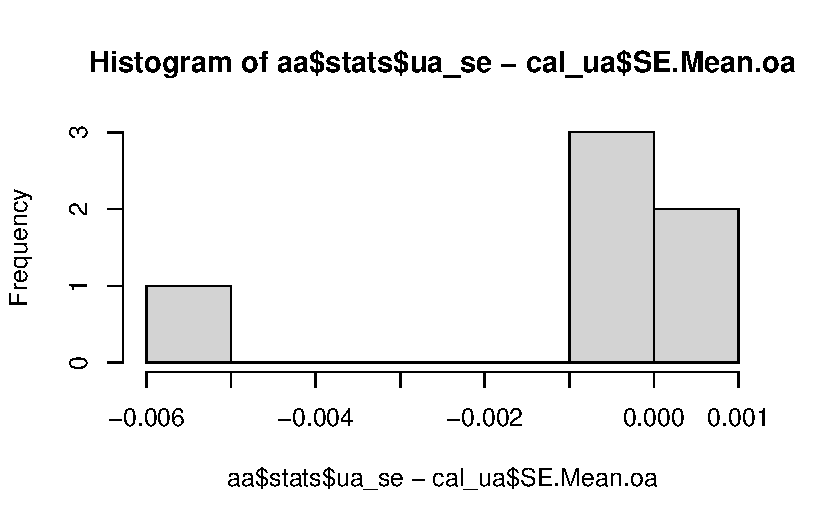
\includegraphics{accuracy_files/figure-pdf/accuracy_regenesees-1.pdf}

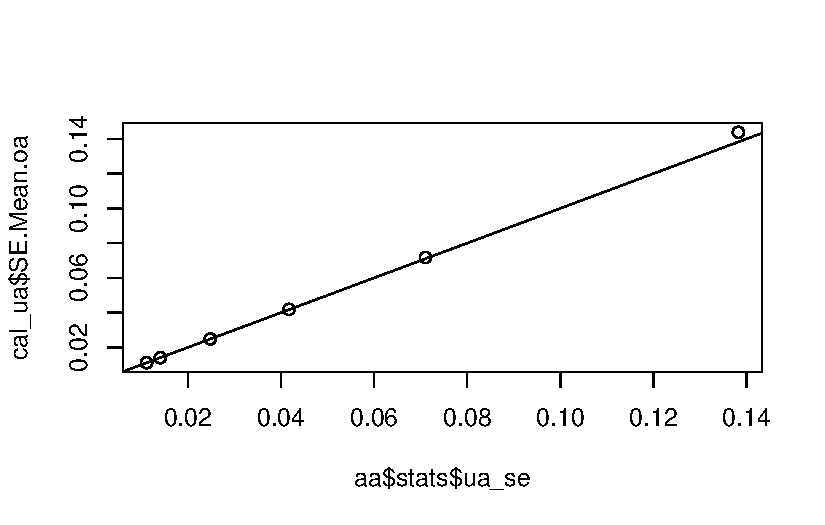
\includegraphics{accuracy_files/figure-pdf/accuracy_regenesees-2.pdf}

\begin{verbatim}
v No differences
\end{verbatim}

\begin{verbatim}
v No differences
\end{verbatim}

\begin{figure}

\centering{

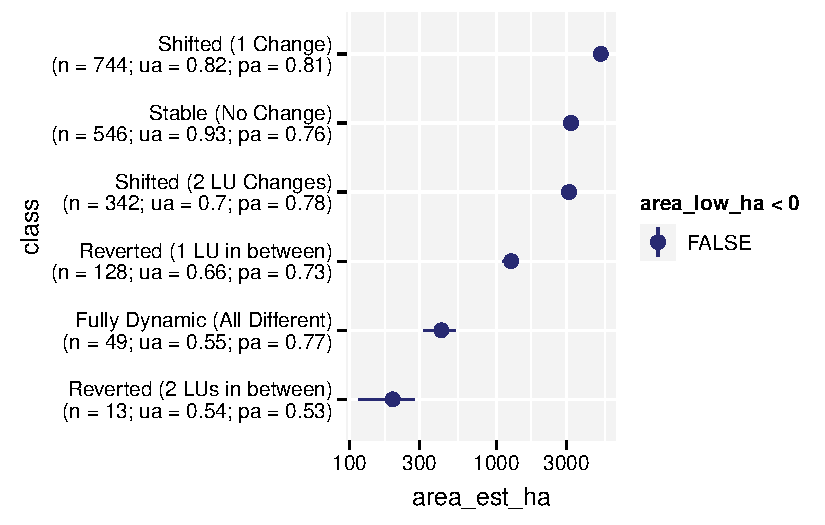
\includegraphics{accuracy_files/figure-pdf/fig-UA_PA-1.pdf}

}

\caption{\label{fig-UA_PA}UA and PA based on the Regenesees package.}

\end{figure}%




\end{document}
